\documentclass[12pt,a4paper]{report}

% -------------------- ENCODING / LANGUAGE --------------------
\usepackage[T1]{fontenc}
\usepackage[utf8]{inputenc}
\usepackage[english]{babel}
\usepackage{indentfirst}

% -------------------- PAGE GEOMETRY --------------------
\usepackage[a4paper,top=2.3cm,bottom=2.5cm,left=3cm,right=2.5cm]{geometry}
\usepackage{ragged2e}

% -------------------- PDF / GRAPHICS --------------------
\usepackage{pdfpages}
\usepackage{graphicx}
\usepackage{float}
\usepackage{subcaption}

% -------------------- MATH --------------------
\usepackage{amsmath,amssymb,amsfonts}

% -------------------- TABLES --------------------
\usepackage{array}
\usepackage{booktabs}
\usepackage{longtable}
\usepackage{tabularx}
\usepackage{float}

% -------------------- LISTS --------------------
\usepackage{enumitem}

% -------------------- COLORS --------------------
\usepackage{xcolor}

% -------------------- CODE --------------------
\usepackage{listings}

% -------------------- DIAGRAMS --------------------
\usepackage{tikz}
\usetikzlibrary{arrows.meta,positioning,shapes.geometric}

% -------------------- CAPTIONS --------------------
\usepackage{caption}

% -------------------- SPACING --------------------
\usepackage{setspace}

% -------------------- HEADER / FOOTER --------------------
\usepackage{fancyhdr}

% -------------------- TOC --------------------
\usepackage{tocloft}

% -------------------- LINKS --------------------
\usepackage{hyperref}

% -------------------- TITLE CONTROL --------------------
\usepackage{titlesec}
% Local width adjustment for selective indentation
\usepackage{changepage}

% Reduce occasional "Overfull \hbox" by allowing small line stretch
\setlength{\emergencystretch}{2em}
% Use \sloppy globally to relax line-breaking (minimal visual impact)
\sloppy
% -------------------- HYPERREF SETUP --------------------
\hypersetup{
    colorlinks=true,
    linkcolor=black,
    filecolor=black,
    urlcolor=blue,
    citecolor=black,
    pdftitle={CyberScope},
    pdfauthor={Mohamed Guizani},
    pdfsubject={End-of-Studies Internship Report},
    pdfkeywords={Web Security, Vulnerability Scanner, React, Node.js, Automation}
}

% -------------------- PAGE BEHAVIOR --------------------
% Avoid stretching vertical whitespace on sparse pages.
\raggedbottom

% -------------------- LINE SPACING --------------------
\onehalfspacing

% -------------------- PARAGRAPH STYLE --------------------
\setlength{\parindent}{1.2cm}
\setlength{\parskip}{0pt}

% -------------------- CAPTION STYLE --------------------
% RULE: Table captions should be placed ABOVE the table
% RULE: Figure captions should be placed BELOW the figure
\captionsetup{
    font=small,
    labelfont=bf,
    justification=centering
}

% -------------------- LIST SPACING --------------------
\setlist[itemize]{topsep=4pt,itemsep=2pt}
\setlist[enumerate]{topsep=4pt,itemsep=2pt}

% -------------------- CODE COLORS --------------------
\definecolor{codebg}{RGB}{245,245,245}
\definecolor{codecomment}{RGB}{0,128,0}
\definecolor{codekeyword}{RGB}{0,0,180}
\definecolor{codestring}{RGB}{163,21,21}

% -------------------- GENERAL LISTING STYLE --------------------
\lstdefinestyle{cyberscope}{
    backgroundcolor=\color{codebg},
    basicstyle=\ttfamily\small,
    breaklines=true,
    captionpos=b,
    commentstyle=\color{codecomment},
    frame=single,
    keepspaces=true,
    keywordstyle=\color{codekeyword}\bfseries,
    numbers=left,
    numbersep=8pt,
    numberstyle=\tiny\color{gray},
    showspaces=false,
    showstringspaces=false,
    showtabs=false,
    stringstyle=\color{codestring},
    tabsize=2
}

% -------------------- JAVASCRIPT --------------------
\lstdefinelanguage{JavaScript}{
    keywords={const, let, var, function, return, async, await, if, else, for, while, break, continue, try, catch, throw, new, class, extends, import, from, export, default},
    keywordstyle=\color{codekeyword}\bfseries,
    ndkeywords={true, false, null, undefined},
    ndkeywordstyle=\color{magenta}\bfseries,
    sensitive=true,
    comment=[l]{//},
    morecomment=[s]{/*}{*/},
    commentstyle=\color{codecomment},
    morestring=[b]",
    morestring=[b]',
    stringstyle=\color{codestring}
}

% -------------------- BASH --------------------
\lstdefinelanguage{Bash}{
    keywords={echo, cd, ls, npm, node, python, pip, curl, nmap, nikto},
    keywordstyle=\color{codekeyword}\bfseries,
    sensitive=true,
    comment=[l]{\#},
    commentstyle=\color{codecomment},
    morestring=[b]",
    morestring=[b]',
    stringstyle=\color{codestring}
}

% -------------------- PYTHON --------------------
\lstdefinelanguage{Python}{
    keywords={def, return, if, elif, else, for, while, break, continue, import, from, as, class, try, except, finally, with, lambda, yield, True, False, None},
    keywordstyle=\color{codekeyword}\bfseries,
    sensitive=true,
    comment=[l]{\#},
    commentstyle=\color{codecomment},
    morestring=[b]",
    morestring=[b]',
    stringstyle=\color{codestring}
}

% -------------------- DEFAULT LISTING STYLE --------------------
\lstset{style=cyberscope}

% -------------------- TOC STYLE --------------------
\renewcommand{\cfttoctitlefont}{\hfill\Large\bfseries}
\renewcommand{\cftaftertoctitle}{\hfill}
\renewcommand{\cftchapfont}{\bfseries}
\renewcommand{\cftchappagefont}{\bfseries}
\setlength{\cftbeforechapskip}{8pt}
\setlength{\cftbeforesecskip}{2pt}
\setlength{\cftbeforesubsecskip}{1pt}
\renewcommand{\cftdotsep}{1}
\setcounter{tocdepth}{2}

% -------------------- HEADER / FOOTER --------------------
\pagestyle{fancy}
\fancyhf{}
\setlength{\headheight}{14.5pt}
\fancyhead[L]{\nouppercase{\leftmark}}
\fancyfoot[C]{\thepage}
\renewcommand{\headrulewidth}{0.4pt}

% -------------------- CHAPTER MARK --------------------
\renewcommand{\chaptermark}[1]{\markboth{Chapter \thechapter.\ #1}{}}

% -------------------- CHAPTER / SECTION STYLES --------------------
\titleformat{\chapter}[display]
  {\normalfont\bfseries}
  {Chapter \thechapter}
  {0.5ex}
  {\Huge}
  []

\titlespacing*{\chapter}{0pt}{-20pt}{10pt}
\titlespacing*{\section}{0pt}{8pt}{4pt}
\titlespacing*{\subsection}{0pt}{6pt}{3pt}

\begin{document}

% -------------------- COVER PAGE --------------------

\includepdf[pages=1]{uploads/page de garde.pdf}

% -------------------- FRONT MATTER --------------------
\clearpage
\pagenumbering{roman}
\setcounter{page}{1}

% -------- Dedication --------
\thispagestyle{plain}
\begin{center}
    {\Large \textbf{Dedications}}
\end{center}

\vspace*{0.6cm}



First and foremost, I thank Allah, the Most Gracious and the Most Merciful, for granting me strength, patience, and perseverance throughout this journey. Without His guidance and blessings, this work would not have been possible.

I dedicate this work with deep love and gratitude to my beloved parents.

To my mother Anissa, for her endless love, sacrifices, encouragement, and prayers that have always been my source of motivation and comfort.

To my father Hassen, for his constant support, wisdom, and efforts to provide me with the best opportunities and guide me toward success.

To my dear siblings, for their encouragement, understanding, and the joy and strength they bring into my life.

This achievement is not mine alone; it is the result of your unconditional support, trust, and love.

Thank you for always believing in me.

\vfill

\hfill \textit{Alhamdulillahi rabbil alameen.}

% -------- Acknowledgements --------
\clearpage
\thispagestyle{plain}
\begin{center}
    {\Large \textbf{Acknowledgments}}
\end{center}

\vspace{0.6cm}

I would like to express my deepest gratitude to all those who have contributed to the completion of this thesis.

\vspace{0.3cm}

First and foremost, I extend my heartfelt appreciation to \textbf{M.\ Yassine Lassoed}, my professional supervisor, who believed in me and in this project from the very beginning. Despite the challenges faced during this internship, he provided me with essential guidance and constant support, enabling me to bring this project to life. His encouragement and trust in my abilities have been invaluable throughout this journey.

\vspace{0.3cm}

I would also like to sincerely thank \textbf{M.\ Mohamed Amine Ben Amar}, my academic supervisor, for his continuous support and valuable advice. Throughout this challenging period, he offered insightful feedback, motivation, and understanding, which greatly contributed to the successful completion of this work.

\vspace{0.3cm}

I am equally grateful to all the individuals who supported me, directly or indirectly, during the realization of this project. Their encouragement and assistance played a significant role in achieving this accomplishment.

\vspace{0.8cm}

\hfill \textit{Thank you for making this achievement possible.}

% -------- Table of Contents --------
\clearpage
\cleardoublepage
\phantomsection
\thispagestyle{plain}

\renewcommand{\contentsname}{Table of Contents}
\tableofcontents

% -------- List of Abbreviations --------
\clearpage
\chapter*{List of Abbreviations}

\begin{tabular}{ll}
API & Application Programming Interface \\
CSP & Content Security Policy \\
JWT & JSON Web Token \\
SPA & Single Page Application \\
SQLi & SQL Injection \\
XSS & Cross-Site Scripting \\
OWASP & Open Worldwide Application Security Project \\
UI & User Interface \\
DB & Database \\
HTTP & Hypertext Transfer Protocol \\
\end{tabular}

% -------- List of Figures --------
\clearpage
\listoffigures
\thispagestyle{plain}

% -------- List of Tables --------
\clearpage
\listoftables
\thispagestyle{plain}

% -------------------- MAIN MATTER --------------------
\clearpage
\pagenumbering{arabic}
\setcounter{page}{1}

% -------- Introduction --------
\chapter*{Introduction}
\addcontentsline{toc}{chapter}{Introduction}
\markboth{Introduction}{Introduction}
\hspace*{1.2cm} In recent years, the rapid evolution of web technologies has significantly transformed the development and deployment of modern applications. Web applications have become increasingly dynamic, interactive, and complex, relying heavily on client-side rendering and continuous communication with backend services. While these advancements have enhanced user experience, they have also expanded the attack surface and introduced new security challenges.

Web application security has become a critical concern for organizations. Vulnerabilities such as SQL injection, cross-site scripting (XSS), and authentication flaws remain among the most exploited attack vectors, as highlighted by the OWASP Top 10. These vulnerabilities can lead to severe consequences, including data breaches, financial losses, and reputational damage.

To mitigate these risks, various security scanning tools have been developed, including solutions such as Nikto, OWASP ZAP, and Burp Suite. Although these tools provide valuable capabilities, they exhibit significant limitations. In particular, traditional scanners struggle to effectively analyze modern Single Page Applications (SPAs), where content is dynamically generated through JavaScript. Furthermore, they often produce redundant or low-priority findings, making vulnerability analysis more complex and less efficient.

In this context, there is a growing need for more intelligent and adaptive security auditing systems capable of handling modern web architectures while improving detection accuracy and result relevance.

To address these challenges, this project introduces \textbf{CyberScope}, an automated web application security auditing system designed to detect and analyze vulnerabilities through intelligent orchestration and advanced automation techniques. The proposed system integrates multiple security tools within a unified pipeline and enhances their capabilities through a browser-based crawling agent capable of exploring dynamic applications. In addition, an AI-driven correlation engine is employed to normalize, deduplicate, and prioritize detected vulnerabilities, providing more meaningful and actionable insights.

The objective of this work is to design and implement a comprehensive and efficient security auditing platform that improves vulnerability detection coverage  and adapts to the complexity of modern web environments.

% -------- Chapter 1 --------
\chapter{General Presentation of the Project}
\section{Introduction}

\justifying
This chapter focuses on the general context of the project. It presents the background of the work, the security challenges faced by modern web applications, the limitations of existing solutions, and the motivation behind the proposed system, \textbf{CyberScope}.

\section{Presentation of the Host Organization}

\justifying
Ernst \& Young (EY)~\cite{ey} is one of the world's leading professional services firms, recognized globally for its expertise in assurance, consulting, strategy, tax, and transaction services. Founded in 1989 through the merger of Ernst \& Whinney and Arthur Young, EY operates in more than 150 countries and employs hundreds of thousands of professionals worldwide.

\indent In Tunisia, EY plays a key role in supporting organizations in their digital transformation and technological innovation. The firm assists both public and private institutions in addressing complex business challenges by providing tailored consulting services and advanced technical solutions.

\indent EY Tunisia offers a wide range of services, including IT consulting, cybersecurity, risk management, and digital innovation. In particular, the firm contributes to strengthening information systems security by identifying vulnerabilities and implementing robust protection mechanisms.

\indent Through its global network and local expertise, EY promotes best practices in cybersecurity and technological development. Its commitment to quality and innovation makes it an ideal environment for the development of advanced solutions such as automated web security auditing systems.

\subsection{EY at the International Level}

\indent At the international level, EY operates as a global professional services network that supports organizations across multiple industries. Its services cover assurance, consulting, tax, strategy, and transaction advisory. Through this worldwide presence, EY assists clients in improving their operational performance, managing risks, and adopting innovative technological solutions.

\indent In the context of digital transformation, EY places strong emphasis on technology, data protection, governance, and cybersecurity. The firm helps organizations address emerging digital risks and adapt to increasingly complex regulatory and technological environments.

\subsection{EY Tunisia and the Cybersecurity Division}

\indent EY Tunisia contributes to the digital transformation of Tunisian organizations by providing consulting and technology-oriented services. Its activities include IT consulting, risk management, cybersecurity, audit, and support for innovation projects.

\indent The cybersecurity division focuses on helping organizations identify weaknesses in their information systems, assess risks, and improve their security posture. This includes activities such as vulnerability assessment, security auditing, governance support, and the implementation of protection strategies. This professional context is directly aligned with the objective of this project, which aims to design an automated and intelligent web application security auditing system.

\vspace{0.6cm}

\noindent Figure~\ref{fig:ey-logo} presents the EY Tunisia organizational context and cybersecurity division, which hosted the development of the CyberScope project.

\vspace{0.3cm}

\begin{figure}[H]
    \centering
    
\includegraphics[width=0.35\textwidth]{uploads/logos/EY_logo.png}
    \caption{EY Tunisia}
    \label{fig:ey-logo}
\end{figure}

\section{Project Context and Problem Statement}

\justifying
With the increasing reliance on web applications in critical domains such as finance, e-commerce, and healthcare, ensuring their security has become a major challenge. Modern applications are more dynamic and complex, which significantly increases their exposure to various cyber threats such as SQL injection, cross-site scripting, and authentication vulnerabilities.

\indent Despite the availability of several security tools, existing solutions often fail to effectively analyze modern web applications, especially those based on dynamic architectures. These tools may miss critical vulnerabilities, generate redundant results, or require significant manual intervention, which reduces their efficiency and reliability.

\indent In this context, the main problem addressed in this project is the lack of an intelligent and automated solution capable of efficiently auditing modern web applications while improving vulnerability detection accuracy and reducing false positives.

\indent The objective of this project is therefore to design and develop \textbf{CyberScope}, an advanced web application security auditing system that enhances vulnerability detection through intelligent orchestration, automation, and improved analysis of security findings.

\section{Overview of Web Application Security}

\justifying
Web application security refers to the set of measures and practices implemented to protect web applications from vulnerabilities and cyber threats. As web applications become increasingly central to business operations and data management, ensuring their security is essential to preserve the confidentiality, integrity, and availability of information.

\indent Modern web applications are exposed to a wide range of attacks that exploit weaknesses in their design, implementation, or configuration. These attacks may target input validation, authentication mechanisms, session management, or communication between client and server. As a result, a single vulnerability can compromise the entire system and lead to severe consequences such as data breaches, financial loss, or reputational damage.

\indent To mitigate these risks, security must be integrated throughout the entire development lifecycle. This includes secure coding practices, regular vulnerability assessments, and the use of automated security tools capable of identifying potential weaknesses before they are exploited.

\indent In this context, standards such as the OWASP Top 10 provide valuable guidance by identifying the most critical web application security risks~\cite{owasp}. These references help developers and security professionals prioritize their efforts and implement effective protection strategies.

\subsection{OWASP Top 10 and Modern Threat Landscape}

\indent The OWASP Top 10 is a widely recognized standard that identifies the most critical security risks affecting web applications~\cite{owasp}. It provides a prioritized list of vulnerabilities such as injection attacks, broken authentication, sensitive data exposure, and cross-site scripting.

\indent These vulnerabilities represent the most common attack vectors exploited by attackers in real-world scenarios. As web technologies evolve, the threat landscape continues to expand, with modern applications introducing new risks related to client-side execution, APIs, and complex system interactions.

\indent By highlighting the most significant threats, the OWASP Top 10 helps developers and security professionals focus on the most impactful vulnerabilities and adopt effective mitigation strategies.

\vspace{0.4cm}

\noindent Table~\ref{tab:owasp-top10} lists the ten most critical web application security risks defined by OWASP, providing a foundation for understanding the primary threats addressed by CyberScope.

\vspace{0.3cm}

\begin{table}[H]
    \centering
    \caption{OWASP Top 10 Web Application Security Risks}
    \label{tab:owasp-top10}
    \renewcommand{\arraystretch}{1.25}
    \begin{tabularx}{\textwidth}{|p{2cm}|X|}
        \hline
        \textbf{ID} & \textbf{Category} \\
        \hline
        A01 & Broken Access Control \\
        \hline
        A02 & Cryptographic Failures \\
        \hline
        A03 & Injection \\
        \hline
        A04 & Insecure Design \\
        \hline
        A05 & Security Misconfiguration \\
        \hline
        A06 & Vulnerable and Outdated Components \\
        \hline
        A07 & Identification and Authentication Failures \\
        \hline
        A08 & Software and Data Integrity Failures \\
        \hline
        A09 & Security Logging and Monitoring Failures \\
        \hline
        A10 & Server-Side Request Forgery \\
        \hline
    \end{tabularx}
\end{table}

\subsection{Statistics and Economic Impact of Web Vulnerabilities}

\indent The impact of web application vulnerabilities is not limited to technical compromise. Security incidents can also lead to financial losses, service disruption, legal consequences, and reputational damage. According to IBM's Cost of a Data Breach Report 2024, the global average cost of a data breach reached USD 4.88 million, representing a significant increase compared to the previous year~\cite{ibm_breach_2024}.

\indent In addition, the Verizon Data Breach Investigations Report highlights the importance of vulnerability exploitation as a major attack vector in real-world incidents~\cite{verizon_dbir_2024}. This shows that unpatched weaknesses and exposed web services remain attractive targets for attackers.

\indent These findings confirm the need for proactive and continuous web application security auditing. Automated solutions can help organizations identify vulnerabilities earlier, reduce remediation delays, and limit the potential impact of security incidents.

\subsection{Limitations of Traditional Vulnerability Scanners}

\indent Traditional vulnerability scanners are widely used to detect security flaws in web applications through automated analysis and predefined signatures. While these tools are effective for identifying known vulnerabilities, they present several limitations when applied to modern web environments.

\indent In particular, they often struggle to analyze dynamic applications, especially those based on client-side rendering and asynchronous communication. As a result, important attack surfaces may remain unexplored. Additionally, these tools may generate a high number of false positives and redundant findings, which complicates the analysis process and reduces their overall efficiency.

\indent These limitations highlight the need for more advanced and intelligent approaches to web application security auditing.

\section{Study of Existing Solutions}

\indent Several tools have been developed to identify vulnerabilities in web applications and assist security professionals in detecting potential threats. These tools provide different approaches to vulnerability scanning, ranging from simple automated checks to advanced interactive analysis. Among the most widely used solutions are Nikto, OWASP ZAP, and Burp Suite.

\subsection{Nikto}

\indent Nikto is an open-source web server scanner designed to detect known vulnerabilities, outdated software, and misconfigurations in web servers~\cite{nikto}. It performs comprehensive checks against a large database of known issues and is commonly used for quick security assessments.

\indent However, Nikto is limited to server-side analysis and does not effectively handle modern dynamic web applications, which reduces its applicability in complex environments.

\vspace{0.4cm}

\noindent Figure~\ref{fig:nikto-logo} represents Nikto logo  .

\vspace{0.3cm}

\begin{figure}[H]
    \centering
    
\includegraphics[height=2cm]{uploads/logos/NIKTOlogo.png}
    \caption{Nikto}
    \label{fig:nikto-logo}
\end{figure}

\subsection{OWASP ZAP}

\indent OWASP ZAP is a widely used open-source security testing tool that provides automated scanning as well as manual testing capabilities~\cite{zap}. It is capable of detecting a variety of vulnerabilities such as injection flaws and security misconfigurations.

\indent Despite its flexibility, ZAP may require proper configuration and user expertise to achieve optimal results, and it can produce a significant number of false positives in complex applications.

\vspace{0.4cm}

\noindent Figure~\ref{fig:zap-logo} represents OWASP ZAP Logo .

\vspace{0.3cm}

\begin{figure}[H]
    \centering
    
\includegraphics[height=2cm]{uploads/logos/ZAPlogo.png}
    \caption{OWASP ZAP}
    \label{fig:zap-logo}
\end{figure}

\subsection{Burp Suite}

\indent Burp Suite is a professional web security testing platform offering a comprehensive set of tools for vulnerability detection and exploitation~\cite{burp}. It allows detailed analysis of HTTP requests and responses and supports advanced manual testing techniques.

\indent While powerful, Burp Suite is more complex to use and often requires significant manual intervention, which can make the testing process time-consuming.

\vspace{0.4cm}

\noindent Figure~\ref{fig:burp-logo} represents Burp Suite logo  .

\vspace{0.3cm}

\begin{figure}[H]
    \centering
    
\includegraphics[height=2cm]{uploads/logos/BURPlogo.png}
    \caption{Burp Suite}
    \label{fig:burp-logo}
\end{figure}

\subsection{AI-Driven Security Testing Solutions}

\indent Recent security testing platforms have started integrating artificial intelligence and advanced automation in order to improve vulnerability detection, prioritization, and remediation guidance. Examples include solutions such as StackHawk, Detectify, and Snyk~\cite{stackhawk,detectify,snyk}.

\indent StackHawk focuses on modern Dynamic Application Security Testing and integration into CI/CD pipelines, allowing development teams to detect vulnerabilities earlier in the software lifecycle. Detectify provides attack surface monitoring and application scanning capabilities, helping organizations continuously discover and assess exposed assets. Snyk focuses on identifying vulnerabilities in code, dependencies, containers, and infrastructure-as-code.

\indent Although these solutions introduce valuable automation and intelligence, they do not fully address the specific objective of this project: building a local, customizable, multi-tool orchestration platform capable of combining dynamic crawling, result deduplication, AI-based interpretation, and professional reporting within a unified workflow.

\subsection{Comparative Analysis}

\indent To better evaluate the strengths and limitations of the studied tools, a comparative analysis is presented below. Although Nikto, OWASP ZAP, and Burp Suite are widely used in web application security testing, each of them addresses only part of the overall auditing process.

\indent Nikto is well suited for rapid server-side checks, OWASP ZAP provides a balanced approach between automation and usability, and Burp Suite offers advanced manual testing capabilities. However, none of these tools fully combines intelligent automation, deep dynamic exploration, and effective reduction of noisy findings.

\vspace{0.5cm}

\noindent Table~\ref{tab:comparative-analysis} provides a detailed comparison of Nikto, OWASP ZAP, Burp Suite, and AI-driven solutions across key criteria, demonstrating that none fully address the integrated orchestration and intelligent analysis required by modern security auditing.

\vspace{0.3cm}

\begin{table}[H]
    \centering
    \caption{Comparative analysis of existing solutions}
    \label{tab:comparative-analysis}
    \renewcommand{\arraystretch}{1.25}
    \begin{tabularx}{\textwidth}{|p{2.8cm}|X|X|X|X|}
        \hline
        \textbf{Criteria} & \textbf{Nikto} & \textbf{OWASP ZAP} & \textbf{Burp Suite} & \textbf{AI-driven Solutions} \\
        \hline
        Type & Open-source server scanner & Open-source proxy and scanner & Professional security testing suite & Automated security platforms \\
        \hline
        Main approach & Signature-based scanning & Automated and manual testing & Advanced manual and automated testing & Continuous testing and prioritization \\
        \hline
        Dynamic application support & Limited & Partial & Good & Good depending on platform \\
        \hline
        AI-assisted analysis & No & Limited & Limited & Yes \\
        \hline
        False positives & High & Medium & Low to medium & Reduced through prioritization \\
        \hline
        Manual testing support & No & Yes & Advanced & Limited to platform features \\
        \hline
        Automation level & High & High & Medium & High \\
        \hline
        Local customization & High & High & Medium & Limited in cloud-based platforms \\
        \hline
        Best suited for & Quick server checks & General web security testing & Deep vulnerability analysis & Continuous security monitoring \\
        \hline
    \end{tabularx}
\end{table}

\indent This comparison shows that existing tools provide useful but incomplete capabilities. Their limitations in terms of automation, adaptability, dynamic analysis, and contextual interpretation justify the need for a more integrated and intelligent solution such as \textbf{CyberScope}.

\section{Critique of Existing Solutions}

\indent Although existing tools such as Nikto, OWASP ZAP, and Burp Suite provide valuable support for vulnerability detection, they still present several limitations when applied to modern web applications.

\indent These limitations are mainly related to the lack of support for dynamic applications, the generation of false positives, and the need for manual intervention. In addition, the absence of intelligent correlation between detected vulnerabilities reduces the clarity and efficiency of the analysis process.

\vspace{0.5cm}

\noindent Table~\ref{tab:limitations-synthesis} synthesizes the main limitations of existing vulnerability scanning tools across dimensions of dynamic application support, false positive rates, correlation capabilities, and scalability.

\vspace{0.3cm}

\begin{table}[H]
    \centering
    \caption{Synthesis of limitations of existing solutions}
    \label{tab:limitations-synthesis}
    \renewcommand{\arraystretch}{1.3}
    \begin{tabularx}{\textwidth}{|p{4cm}|X|X|}
        \hline
        \textbf{Limitation} & \textbf{Description} & \textbf{Impact} \\
        \hline
        Limited support for dynamic applications & Difficulty handling JavaScript-based applications & Incomplete vulnerability detection \\
        \hline
        High false positives & Redundant or irrelevant findings & Time-consuming analysis \\
        \hline
        Lack of intelligent correlation & No prioritization of vulnerabilities & Reduced clarity of results \\
        \hline
        Manual intervention required & Dependence on user expertise & Low scalability \\
        \hline
        Fragmented tool usage & Multiple tools used separately & Complex workflow \\
        \hline
    \end{tabularx}
\end{table}

\indent These limitations highlight the need for a more advanced solution capable of combining automation, accuracy, and adaptability.




\section{Proposed Solution: CyberScope}




\indent To overcome the limitations identified in existing solutions, this project proposes \textbf{CyberScope}, an intelligent web application security auditing system.

\indent CyberScope is based on a unified architecture that integrates multiple security tools into a single automated pipeline. It introduces a browser-based crawling mechanism capable of exploring modern dynamic applications and interacting with client-side components.

\indent In addition, the system incorporates an intelligent analysis layer responsible for normalizing, deduplicating, and prioritizing vulnerabilities. This significantly reduces noise and improves the relevance of the results.

\indent By combining automation, dynamic exploration, and intelligent processing, CyberScope aims to provide a more efficient and scalable approach to web application security auditing.

\noindent Figure~\ref{fig:cyberscope-logo} presents the CyberScope system logo .

\begin{figure}[H]
    \centering
    
\includegraphics[width=0.22\textwidth]{uploads/logos/logo.png}
    \caption{CyberScope Logo}
    \label{fig:cyberscope-logo}
\end{figure}


\subsection{Vision and Objectives}

\indent The vision of \textbf{CyberScope} is to provide an enterprise-oriented web application security auditing platform that helps security analysts detect, understand, and prioritize vulnerabilities more efficiently. To realize this vision, the platform automates the coordinated execution of multiple open-source security tools within a unified workflow, improves coverage of modern dynamic applications through browser-driven exploration, and reduces duplicated or noisy findings via normalization and deduplication. An AI-assisted analysis layer produces clearer vulnerability interpretations and risk prioritization, and results are delivered through a professional dashboard with automated, structured audit reports for stakeholders.

\subsection{Contributions and Added Value Compared to Existing Solutions}

\indent CyberScope does not aim to replace existing scanners. Instead, it acts as an intelligent orchestration and analysis layer that enhances their effectiveness by combining their outputs and presenting them in a more structured and actionable form.

\vspace{0.5cm}
\noindent Table~\ref{tab:cyberscope-value} highlights the key contributions of CyberScope compared to existing solutions, demonstrating added value through integrated orchestration, comprehensive dynamic analysis, intelligent result normalization, and AI-assisted interpretation.

\begin{table}[H]
    \centering
    \caption{Added value of CyberScope compared to existing solutions}
    \label{tab:cyberscope-value}
    \renewcommand{\arraystretch}{1.3}
    \begin{tabularx}{\textwidth}{|p{4cm}|X|X|}
        \hline
        \textbf{Aspect} & \textbf{Existing Solutions} & \textbf{CyberScope Contribution} \\
        \hline
        Tool execution & Tools are generally used separately & Unified orchestration of multiple security tools \\
        \hline
        Dynamic analysis & Limited or partial support for modern applications & BrowserAgent for exploring dynamic interfaces and hidden endpoints \\
        \hline
        Result processing & Raw outputs or tool-specific formats & Normalized and deduplicated vulnerability findings \\
        \hline
        Risk interpretation & Mostly technical results requiring manual analysis & AI-assisted interpretation and prioritized remediation guidance \\
        \hline
        Visualization & Basic reports or complex expert interfaces & Structured dashboard and clearer vulnerability presentation \\
        \hline
        Reporting & Often manual or tool-dependent & Automated generation of professional audit reports \\
        \hline
    \end{tabularx}
\end{table}


\section{Conclusion}

\indent This chapter introduced the general context of the project by highlighting the importance of web application security and the challenges posed by modern dynamic applications. It also presented a study of existing solutions and identified their main limitations.

\indent Based on this analysis, the need for a more advanced and intelligent approach was established, leading to the proposal of \textbf{CyberScope}. The next chapter will focus on the analysis of the system requirements and the initialization of the Scrum process.


% -------- Chapter 2 --------
\chapter{System Analysis and Requirements Specification}
\section{Introduction}

\justifying
This chapter presents the analysis and specification of the \textbf{CyberScope} system. It introduces the adopted development methodology, identifies the main stakeholders, presents the development environment, and defines both functional and non-functional requirements. It also presents the use case diagram, the textual description of the main use cases, and the organization of the project through the product backlog and sprint planning.

\section{Adopted Development Methodology}

\justifying
To ensure a flexible and progressive development process, the Scrum methodology was adopted for the realization of \textbf{CyberScope}. Scrum is an agile framework based on iterative development, incremental delivery, continuous feedback, and adaptation to evolving requirements.

{\titlespacing*{\subsection}{1.0cm}{6pt}{3pt}
\subsection{Justification of the Choice of Scrum}
}

\justifying
The choice of Scrum is justified by the nature of the CyberScope project, which involves several heterogeneous components such as a frontend dashboard, a backend API, a Python-based scanning engine, external security tools, and AI-based analysis modules.

A traditional sequential development approach would make it difficult to validate each component progressively. Scrum allows the project to be divided into smaller increments, making it possible to test, validate, and improve each part of the system throughout development; this iterative approach is illustrated in Figure~\ref{fig:scrum-cyberscope}, which shows the sprint cycles, ceremonies, and feedback loops that guided the three project sprints.

\begin{figure}[H]
    \centering
    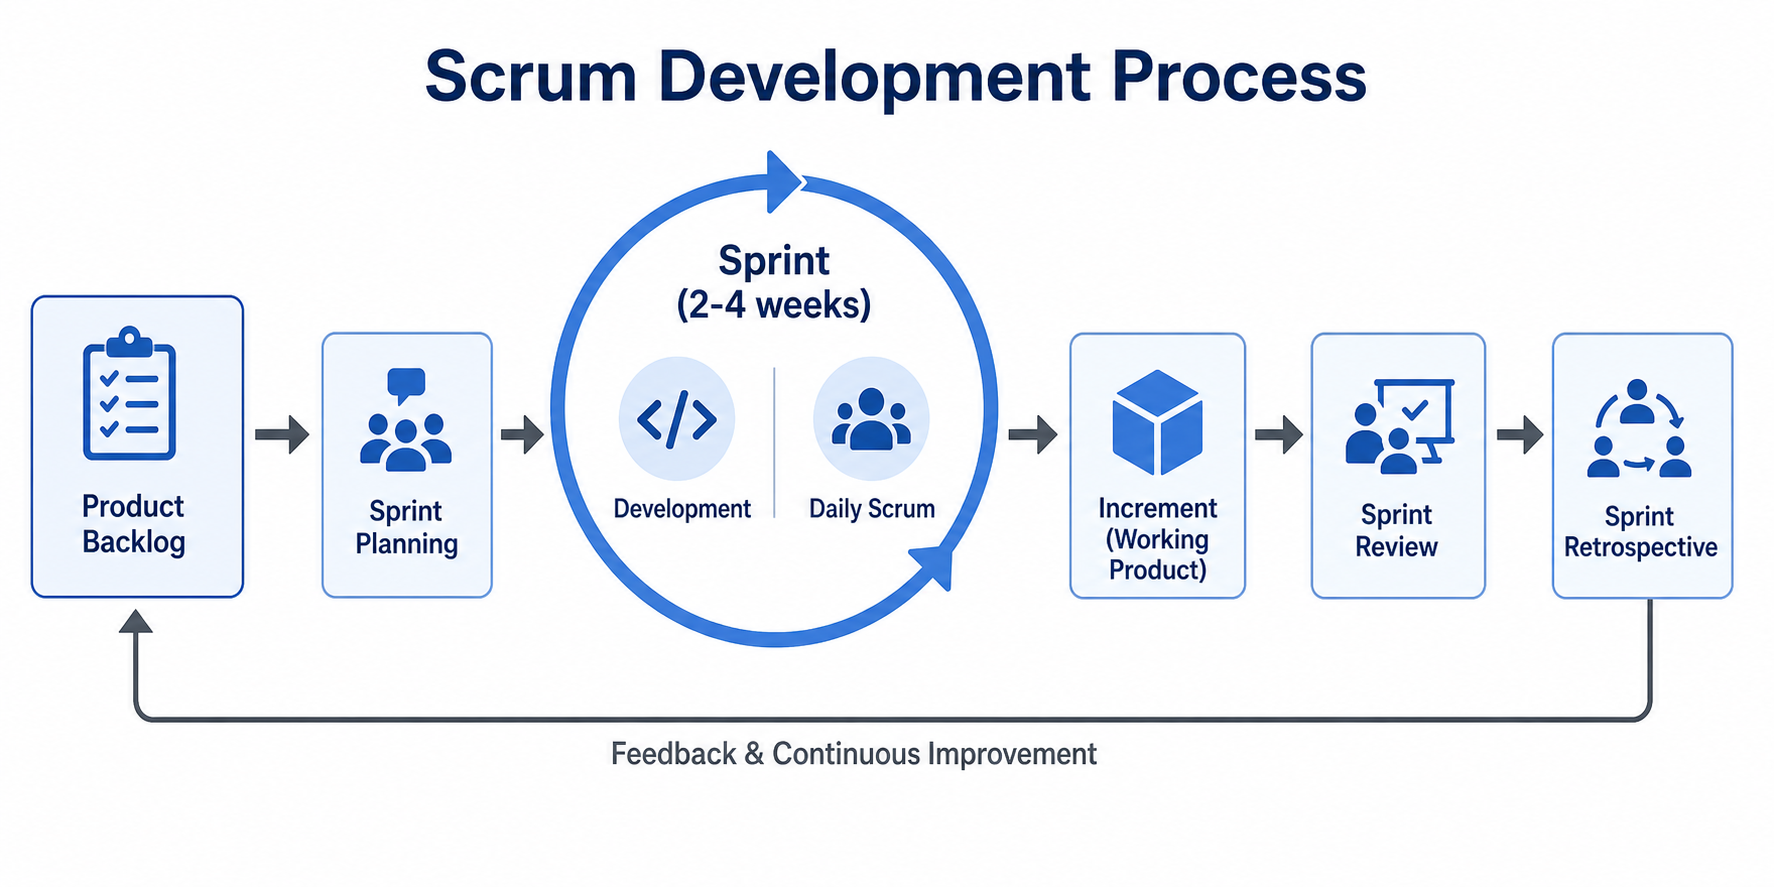
\includegraphics[width=1\textwidth]{uploads/images/scrum.png}
    \caption{Scrum Development Process adapted to CyberScope}
    \label{fig:scrum-cyberscope}
\end{figure}

\subsection{Organization of Sprints }

\vspace{0.4cm}

\indent CyberScope is organized into three iterative sprints, each with distinct objectives and deliverables; each sprint delivers a cohesive set of user stories aligned with its main objective. Table~\ref{tab:sprint-organization} presents the sprint timeline and main goals, showing progress from backend infrastructure through tool integration to attack graph generation over a 12-week development cycle.
\begin{table}[H]
    \centering
    \caption{Sprint Organization of CyberScope}
    \label{tab:sprint-organization}
    \renewcommand{\arraystretch}{1.25}
    \begin{tabularx}{\textwidth}{|p{1.8cm}|X|X|p{1.8cm}|}
        \hline
        \textbf{Sprint} & \textbf{Main Objective} & \textbf{Deliverable} & \textbf{Duration} \\
        \hline
        Sprint 1 & Backend foundation and database setup & Core backend APIs and database structure & 4 weeks \\
        \hline
        Sprint 2 & Scanning engine and tool orchestration & Integration of tools and scanning pipeline & 4 weeks \\
        \hline
        Sprint 3 & Attack Graph Generation & Computational framework for generating attack graphs & 4 weeks \\
        \hline
    \end{tabularx}
    \end{table}


\subsection{Backlog estimation methods}

User stories were estimated using a T‑shirt sizing approach (XS–XL) that favors relative effort over numeric points. This simplifies comparisons of complexity across backlog items; the adopted sizing scale is shown in Figure~\ref{fig:tshirt-sizing}.

\begin{figure}[H]
    \centering
    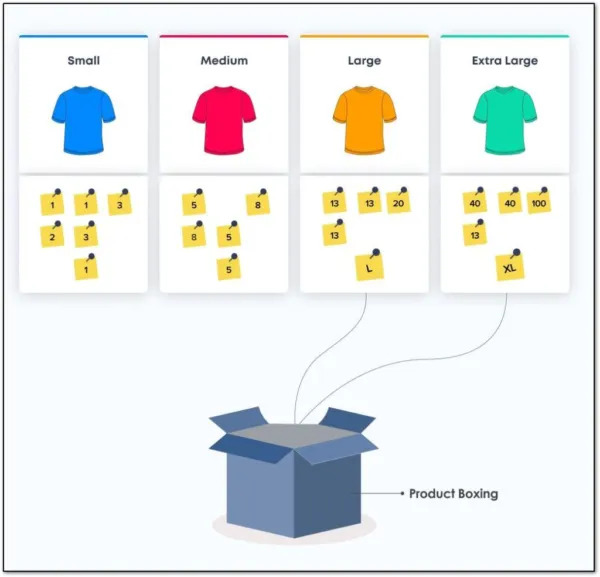
\includegraphics[width=0.6\textwidth]{uploads/images/tshirt (1).jpg}
    \caption{T-shirt sizing method (XS--XL) used for coarse estimates}
    \label{fig:tshirt-sizing}
\end{figure}
 
\subsection{Product Backlog}

\indent\justifying The product backlog consolidates all identified user stories, features, and technical tasks prioritized for implementation. Table~\ref{tab:product-backlog} lists the backlog items with their assigned sprint, category, and priority, providing a roadmap for development and release planning.


    {\small
    \begin{longtable}{|>{\centering\arraybackslash}p{1.4cm}|>{\centering\arraybackslash}p{2cm}|>{\centering\arraybackslash}p{2.2cm}|>{\raggedright\arraybackslash}p{7.5cm}|>{\centering\arraybackslash}p{1.2cm}|}
        \caption{Product Backlog of CyberScope}
        \label{tab:product-backlog} \\
        \hline
        \textbf{ID} & \textbf{Sprint} & \textbf{Category} & \textbf{User Story} & \textbf{Priority} \\
        \hline
        \endfirsthead
        \multicolumn{5}{c}{\textit{}} \\
        \hline
        \textbf{ID} & \textbf{Sprint} & \textbf{Category} & \textbf{User Story} & \textbf{Priority} \\
        \hline
        \endhead
        \hline
        \multicolumn{5}{r}{\textit{continued on next page}} \\
        \endfoot
        \hline
        \endlastfoot
        US-S1-01 & Sprint 1 & Authentication & As a User, I can create an account and log in to the platform so that I can securely access my data and scanning features. & High \\
        \hline
        US-S1-02 & Sprint 1 & Session & As a Guest User, I can start a temporary guest session without creating a persistent account so that I can quickly evaluate the platform. & Medium \\
        \hline
        US-S1-03 & Sprint 1 & Access Control & As a User, I can access protected pages such as the scanner and scan history so that I can run scans and review past results. & High \\
        \hline
        US-S1-04 & Sprint 1 & Session Management & As the System, I can verify and refresh the current session by exposing the authenticated user profile so that sessions remain valid and secure. & High \\
        \hline
        US-S1-05 & Sprint 1 & Tool Integration & As the System, I must resolve and safely execute HexStrike scanner binaries with timeout enforcement and resource limits so that tool outputs are captured reliably for processing. & High \\
        \hline
        US-S1-06 & Sprint 1 & AI Foundation & As the System, I must integrate Ollama for local AI inference to enable contextual analysis and intelligent recommendation generation without external API dependencies. & High \\
        \hline
        US-S2-01 & Sprint 2 & Scan Submission & As a User, I can submit a scan target (URL) and receive a job identifier so that I can track and retrieve results. & High \\
        \hline
        US-S2-03 & Sprint 2 & Execution & As the System, I can run scanner tools and collect raw outputs so that findings can be processed. & High \\
        \hline
        US-S2-04 & Sprint 2 & Normalization & As the System, I can normalize raw outputs into a unified schema so that results are consistent across tools. & High \\
        \hline
        US-S2-05 & Sprint 2 & Matching & As the System, I can match normalized findings to the vulnerability catalog and assign severities so that results are actionable. & High \\
        \hline
        US-S2-06 & Sprint 2 & Results UI & As a User, I can view, filter, and export scan history and results so that I can analyze and share findings. & Medium \\
        \hline
        US-S2-07 & Sprint 2 & Operations & As the System, I can monitor queue status and worker health so that the processing pipeline remains reliable. & Medium \\
        \hline
        US-S3-01 & Sprint 3 & Scenario Gen & As a User, I can request an attack scenario for a specific vulnerability and receive structured steps and a graph object so that I can investigate exploitation paths. & High \\
        \hline
        US-S3-02 & Sprint 3 & Remediation & As a User, I can click on an attack scenario step in the interactive graph so that I receive contextualized remediation tips and countermeasures to address that specific vulnerability. & High \\
        \hline
        US-S3-03 & Sprint 3 & Normalization & As the System, I must validate and normalize AI responses into a safe, consistent graph payload (nodes/edges) so that frontend rendering is robust and secure. & High \\
        \hline
        US-S3-04 & Sprint 3 & Frontend Integration & As a User, the Dashboard should render the returned graph (React Flow) and allow interaction with attack scenario steps so that I can explore potential attack paths. & Medium \\
        \hline
        US-S3-05 & Sprint 3 & Operations & As the System, I should handle AI timeouts, malformed responses, and return useful error messages so that failures are observable and debuggable. & Medium \\
        \hline
    \end{longtable}
    }
% duplicate/older Product Backlog table removed (kept the sprint-assigned detailed backlog above)



\section{Stakeholder Identification}

\indent The development and use of \textbf{CyberScope} involve three primary actors, each interacting with the system according to specific roles and responsibilities.

\indent The \textbf{User} represents the primary actor and main beneficiary of the platform. This actor performs core activities such as creating an account, logging in, submitting target URLs for security analysis, launching scans, and analyzing results through the interactive dashboard. The User relies on the system to provide accurate vulnerability detection and actionable remediation recommendations.

\indent The \textbf{Guest User} is a secondary actor who interacts with the platform without establishing a persistent account. This actor can access the system through a temporary guest session to evaluate the platform's capabilities and explore basic features, enabling quick evaluation without registration overhead.

\indent The \textbf{System} acts as the backend orchestrator and automated processor.This actor performs critical operations including tool integration and resolution, session management, scan execution and pipeline orchestration, output normalization and enrichment, vulnerability matching, and AI-driven attack graph generation.The System ensures reliable, scalable, and secure operation of all automated processes.
\break
\section{System Overview}

\indent\justifying CyberScope is an intelligent web application security auditing platform designed to automate vulnerability detection and analysis. It integrates multiple security tools into a unified pipeline and provides advanced features such as dynamic crawling, result aggregation, and AI-driven interpretation.

\indent The system is composed of three main components:

\begin{itemize}
    \item A frontend dashboard for user interaction and visualization
    \item A backend orchestration layer managing scans and data
    \item A scanning engine responsible for executing security tools
\end{itemize}

\section{Functional Requirements}

\indent\justifying The functional requirements define the core services provided by CyberScope. These functionalities describe how the system interacts with users and how it performs automated security analysis, from scan initiation to result reporting.

\subsection{Scan Initiation and Target Submission}

\indent The system must allow users to submit a target web application through a valid URL and initiate a security scan. Prior to execution, the system must validate the input to ensure correctness and accessibility of the target.

\indent Once validated, the system must create a scan instance, assign it a unique identifier, and trigger the scanning workflow. The user must be able to monitor the progress of the scan (e.g., pending, running, completed, failed) through the interface. Additionally, the system should support multiple concurrent scans and maintain a history of previous scans for later consultation.

\subsection{Intelligent Tool Orchestration}

\indent CyberScope must coordinate the execution of multiple security tools within a unified and automated pipeline. The system should dynamically orchestrate tools such as Nmap, Nuclei, Nikto, and SQLMap depending on the target characteristics.

\indent The orchestration process must ensure efficient scheduling, avoid redundant executions, and support parallel processing when possible. It must also manage tool configuration, execution, and result collection transparently, without requiring manual user intervention.

\subsection{Dynamic Application Crawling (BrowserAgent)}

\indent The system must include a browser-based crawling component, referred to as the \textbf{BrowserAgent}, capable of interacting with modern web applications.

\indent This component must simulate real user behavior by executing JavaScript, navigating through dynamic interfaces, and capturing network requests. It enables the discovery of hidden endpoints, API calls, and parameters that are not accessible through traditional static scanning techniques.

\indent This functionality is particularly important for analyzing Single Page Applications (SPAs) and dynamically generated content.

\subsection{Vulnerability Detection and Analysis}

\indent The system must detect a wide range of web application vulnerabilities, including SQL injection, cross-site scripting (XSS), exposed services, insecure configurations, and outdated components.

\indent CyberScope must process the outputs of integrated tools and transform them into structured vulnerability objects. Each vulnerability should include detailed information such as its type, severity level, affected endpoint, technical evidence, and potential impact.

\indent This structured representation facilitates further analysis, prioritization, and decision-making.

\subsection{Aggregation and Visualization of Results}

\indent The system must aggregate results collected from multiple tools and eliminate duplicate findings through normalization and deduplication mechanisms.

\indent The processed results must be presented through an intuitive dashboard that allows users to explore vulnerabilities using filters, sorting options, and visual indicators. The interface should provide a clear overview of the security posture, including severity distribution, affected components, and scan statistics.

\indent This improves readability and enables users to quickly identify and prioritize critical issues.

\subsection{Report Generation}

\indent The system must generate comprehensive and structured reports summarizing the results of a security scan.

\indent These reports should include target information, detected vulnerabilities, severity classification, risk assessment, and remediation recommendations. The reports must be exportable in a professional format (e.g., PDF) to facilitate communication with stakeholders and support auditing processes.

\section{Non-Functional Requirements}

\indent Non-functional requirements define the quality attributes and operational constraints of the CyberScope system. They ensure that the platform is efficient, secure, reliable, and maintainable.

\subsection{Performance and Scalability}

\indent The system must provide acceptable performance in terms of response time and processing efficiency. While vulnerability scans may be resource-intensive, user interactions with the platform must remain responsive.

\indent The architecture should support scalability by allowing the distribution of system components (frontend, backend, scanning engine) to handle increasing workloads and larger target applications without significant performance degradation.

\subsection{Security Requirements}

\indent CyberScope must implement strong security mechanisms to protect user data and scan results. Authentication and authorization must be enforced using secure approaches such as JSON Web Tokens (JWT).

\indent Sensitive data must be protected against unauthorized access, and secure communication must be ensured between system components. Given the nature of the platform, maintaining confidentiality and integrity is essential.

\subsection{Usability}

\indent The platform must provide an intuitive and user-friendly interface that simplifies interaction with complex security data.

\indent The dashboard should present information in a clear and structured manner, allowing users to easily navigate between scans, analyze vulnerabilities, and access reports. Important elements such as severity levels and risk indicators should be highlighted to improve decision-making.

\subsection{Reliability and Availability}

\indent The system must ensure stable and reliable operation during scan execution and data processing. It should handle failures gracefully, such as tool crashes or network interruptions, without compromising data integrity.

\indent Appropriate logging and error-handling mechanisms must be implemented to support monitoring and debugging. The system should also maintain high availability with minimal downtime.

\subsection{Maintainability and Extensibility}

\indent CyberScope must be designed using a modular architecture that facilitates maintenance and future evolution.

\indent The system should allow easy integration of new security tools, updates to existing components, and modifications without affecting the overall system stability. Clear separation between components (frontend, backend, scanning engine) enhances maintainability.

\indent Extensibility is essential to adapt the platform to new vulnerabilities, technologies, and evolving security requirements.

\section{Global Use Case Diagram}

\indent The use case diagram illustrates the main interactions between the user and the CyberScope system; Figure~\ref{fig:global-usecase} shows the main actors (User, Guest User, and System) and the primary use case flows for authentication, scanning, and attack scenario generation.

\begin{figure}[H]
    \centering
    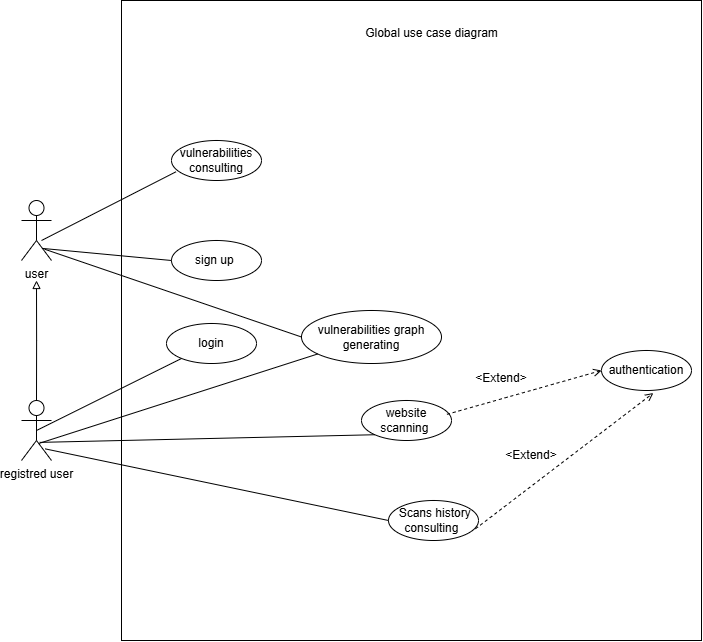
\includegraphics[width=0.85\textwidth]{uploads/diagrams/use case general .drawio.png}
    \caption{Global Use Case Diagram of CyberScope}
    \label{fig:global-usecase}
\end{figure}


\clearpage
\section{Global Class Diagram}


\vspace{0.3cm}

\indent The class diagram presents the main structural components of CyberScope and the relationships between its core services, models, and orchestration layers.
\noindent Figure~\ref{fig:global-class-diagram} presents the principal components and relationships of CyberScope architecture, including frontend models, backend API services, scanning engine, and external tool integration layers.

\begin{figure}[H]
    \centering
    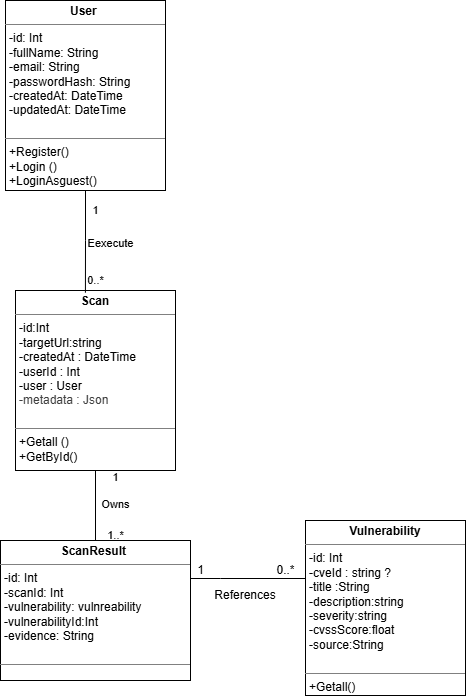
\includegraphics[width=0.8\textwidth]{uploads/diagrams/classglobal.drawio.png}
    \caption{Global Class Diagram of CyberScope}
    \label{fig:global-class-diagram}
\end{figure}

\section{Development Environment}

\indent This section presents the technical environment used to design, implement, and test \textbf{CyberScope}. It highlights the main programming languages, frameworks, tools, and software resources that supported the project.

\subsection{Material Environment}

\indent Development work was performed on a Windows workstation using the following primary tools; Figure~\ref{fig:vscode-logo} shows Visual Studio Code, the primary development environment used for writing frontend and backend code, providing advanced features for debugging and extension management.


\vspace{0.3cm}

\begin{figure}[H]
    \centering
    
\includegraphics[width=2.4cm]{uploads/logos/vscode.png}
    \caption{Logo of Visual Studio Code.}
    \label{fig:vscode-logo}
    \vspace{0.2cm}
    \begin{minipage}{0.9\textwidth}
        \centering
    \end{minipage}
\end{figure}
\indent Figure~\ref{fig:git-logo} represents Git, the distributed version control system used for managing source code, tracking development history, and coordinating collaborative contributions throughout the project lifecycle.

\vspace{0.3cm}
\begin{figure}[H]
    \centering
    
\includegraphics[width=2.4cm]{uploads/logos/git.png}
    \caption{Logo of Git.}
    \label{fig:git-logo}
    \vspace{0.2cm}
    \begin{minipage}{0.9\textwidth}
        \centering
    \end{minipage}
\end{figure}

\indent Figure~\ref{fig:chromium-logo} shows the Chromium/Google Chrome browser, used for manual functional testing, dynamic content verification, and network analysis of the CyberScope frontend during development.

\vspace{0.3cm}
\begin{figure}[H]
    \centering
    
\includegraphics[width=2.4cm]{uploads/logos/Chromium_Logo.png}
    \caption{Logo of Google Chrome / Chromium.}
    \label{fig:chromium-logo}
    \vspace{0.2cm}
    \begin{minipage}{0.9\textwidth}
        \centering
    \end{minipage}
\end{figure}

\indent Figure~\ref{fig:drawio-logo} represents diagrams.net (draw.io), the diagramming tool used to create all architectural diagrams, use case diagrams, class diagrams, and sequence diagrams throughout the documentation.

\vspace{0.3cm}
\begin{figure}[H]

    \centering
    
\includegraphics[width=2.4cm]{uploads/images/drawiologo.png}
    \caption{Logo of diagrams.net (draw.io).}
    \label{fig:drawio-logo}
    \vspace{0.2cm}
    \begin{minipage}{0.9\textwidth}
        \centering
    \end{minipage}
\end{figure}

\indent Figure~\ref{fig:overleaf-logo} shows Overleaf, the online collaborative LaTeX editor used for writing, editing, and compiling the project documentation and technical report.

\vspace{0.3cm}
\begin{figure}[H]
    \centering
    
\includegraphics[width=2.4cm]{uploads/images/overleaf-logo-primary.png}
    \caption{Logo of Overleaf.}
    \label{fig:overleaf-logo}
    \vspace{0.2cm}
    \begin{minipage}{0.9\textwidth}
        \centering
    \end{minipage}
\end{figure}


\subsection{Software Environment}

\indent The software stack is organized by layer; the following items present the main technologies with a short description for each.

\vspace{0.3cm}
\noindent\textbullet\ \textbf{Backend}

\vspace{0.2cm}

\indent Figure~\ref{fig:node-logo} represents Node.js, the JavaScript runtime environment providing the execution platform for the CyberScope backend server and all related processes.

\vspace{0.3cm}

\begin{figure}[H]
    \centering
    
\includegraphics[width=2.2cm]{uploads/logos/node.png}
    \caption{Node.js}
    \label{fig:node-logo}
    \vspace{0.2cm}
    \begin{minipage}{0.9\textwidth}
        \centering
    \end{minipage}
\end{figure}

\vspace{0.3cm}

\indent Figure~\ref{fig:express-logo} shows Express.js, the lightweight web framework used to define all RESTful API endpoints, routing logic, and middleware components in the CyberScope backend.

\vspace{0.3cm}

\begin{figure}[H]
    \centering
    
\includegraphics[width=2.2cm]{uploads/logos/Expressjs.png}
    \caption{Express.js}
    \label{fig:express-logo}
    \vspace{0.2cm}
    \begin{minipage}{0.9\textwidth}
        \centering
    \end{minipage}
\end{figure}

\vspace{0.3cm}


\vspace{0.3cm}
\indent Figure~\ref{fig:prisma-logo} shows Prisma, the Object-Relational Mapping tool providing type-safe database access, migrations, and schema management for the PostgreSQL database.

\begin{figure}[H]
    \centering
    
\includegraphics[width=2.2cm]{uploads/logos/prisma.jpg}
    \caption{Prisma}
    \label{fig:prisma-logo}
    \vspace{0.2cm}
    \begin{minipage}{0.9\textwidth}
        \centering
    \end{minipage}
\end{figure}

\vspace{0.3cm}

\indent Figure~\ref{fig:postgresql-logo} shows PostgreSQL, the robust relational database management system used to persistently store user data, scan jobs, vulnerabilities, and analysis results.

\vspace{0.3cm}

\begin{figure}[H]
    \centering
    
\includegraphics[width=2.2cm]{uploads/logos/postgresql.png}
    \caption{PostgreSQL}
    \label{fig:postgresql-logo}
    \vspace{0.2cm}
    \begin{minipage}{0.9\textwidth}
        \centering
    \end{minipage}
\end{figure}

\vspace{0.4cm}
\noindent\textbullet\ \textbf{Frontend} \\
\vspace{0.15cm}

\indent Figure~\ref{fig:react-logo} represents React, the JavaScript library used to build the interactive CyberScope frontend dashboard with reusable components, state management, and dynamic user interfaces.

\vspace{0.2cm}
\begin{figure}[H]
    \centering
    
\includegraphics[width=2.2cm]{uploads/logos/react.png}
    \caption{React}
    \label{fig:react-logo}
    \vspace{0.2cm}
    \begin{minipage}{0.9\textwidth}
        \centering
    \end{minipage}
\end{figure}


\vspace{0.3cm}

\indent Figure~\ref{fig:vite-logo} shows Vite, the modern frontend build tool and development server used to provide fast hot module replacement and optimized production builds for the React frontend.

\vspace{0.3cm}

\begin{figure}[H]
    \centering
    
\includegraphics[width=2.2cm]{uploads/logos/vite.jpg}
    \caption{Vite}
    \label{fig:vite-logo}
    \vspace{0.2cm}
    \begin{minipage}{0.9\textwidth}
        \centering
    \end{minipage}
\end{figure}

\vspace{0.3cm}

\indent Figure~\ref{fig:typescript-logo} represents TypeScript, the typed superset of JavaScript used throughout both frontend and backend development to provide static type checking and improved code quality.

\vspace{0.3cm}

\begin{figure}[H]
    \centering
    
\includegraphics[width=2.2cm]{uploads/logos/TS.png}
    \caption{TypeScript}
    \label{fig:typescript-logo}
    \vspace{0.2cm}
    \begin{minipage}{0.9\textwidth}
        \centering
    \end{minipage}
\end{figure}

\vspace{0.4cm}
\noindent\textbullet\ \textbf{Scanning \& AI Tools}

\indent Figure~\ref{fig:ollama-logo} shows Ollama, the local AI engine used to assist in analysis and prompt generation within CyberScope.

\vspace{0.3cm}
\begin{figure}[H]
    \centering
    
\includegraphics[width=2.2cm]{uploads/logos/ollama.png}
    \caption{Ollama}
    \label{fig:ollama-logo}
    \vspace{0.2cm}
    \begin{minipage}{0.9\textwidth}
        \centering
    \end{minipage}
\end{figure}
\indent Figure~\ref{fig:hexstrike-logo} shows HexStrike AI, the orchestration layer for automated execution of multiple security tools in CyberScope.

\vspace{0.3cm}
\begin{figure}[H]
    \centering
    
\includegraphics[width=2.2cm]{uploads/logos/hexstrike.png}
    \caption{HexStrike AI}
    \label{fig:hexstrike-logo}
    \vspace{0.2cm}
    \begin{minipage}{0.9\textwidth}
        \centering
    \end{minipage}
\end{figure}

% Diagramming and documentation tools are declared in Material Environment (2.8.1)



\section{Conclusion}

\indent This chapter presented the analysis and specification of the CyberScope system, including the adopted methodology, stakeholder identification, development environment, system overview, and requirements. These elements provide a solid foundation for the system design presented in the next chapter.


% -------- Chapter 3 --------
\chapter{Backend Foundation \& Authentication System}
\section{Introduction}

This sprint focuses on the authentication layer of the HexStrike platform and on the access control rules that protect the main application modules. The goal of this iteration is to provide a secure entry point to the system, manage user sessions with JWT, and restrict sensitive actions such as scan creation and scan history access to authenticated users only.

In practice, this sprint covers the login and registration flow, the guest session mechanism, protected routes on the frontend, and the backend middleware that validates every secured request.

\subsection{Sprint Purpose}

The purpose of this sprint is to secure the platform's entry points and session management to enable safe use of the scanning and analysis features. Concretely, the sprint delivers a robust authentication system, a guest mode for quick evaluation, and middleware that enforces access control for all sensitive API endpoints.

\section{Sprint Backlog}

The backlog of this sprint contains the following user stories:

\begin{table}[H]
    \centering
    \renewcommand{\arraystretch}{1.2}
    \begin{tabularx}{\textwidth}{|X|}
        \hline
        As a visitor, I can create an account and log in to the platform. \\\hline
        As a user, I can start a temporary guest session without creating a persistent account. \\\hline
        As an authenticated user, I can access protected pages such as the scanner and scan history. \\\hline
        As a guest user, I cannot access protected resources or save scans in the database. \\\hline
        As the system, I can verify and refresh the current session by exposing the authenticated user profile. \\\hline
    \end{tabularx}
    \caption{Sprint Backlog}
\end{table}

\section{Requirements Analysis}

\subsection{Use Case Diagram}

The actors involved in this sprint are the visitor, the registered user, and the guest user. The visitor can register and log in, the registered user can access protected modules, and the guest user can only use limited temporary access.

The following figure is reserved for the use case diagram of this sprint.

\begin{figure}[H]
    \centering
    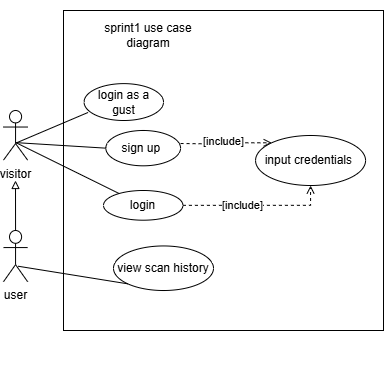
\includegraphics[width=0.85\textwidth]{uploads/diagrams/sprint1usecase.drawio.png}
    \caption{Use case diagram for authentication and access control}
    \label{fig:sprint1-usecase}
\end{figure}

\subsection{Use Case Description}

The main use cases of this sprint are summarized in the following tables.

\begin{table}[H]
    \centering
    \renewcommand{\arraystretch}{1.2}
    \begin{tabular}{|p{3cm}|p{11cm}|}
        \hline
        \textbf{Use case} & Register \\ \hline
        \textbf{Actor} & Visitor \\ \hline
        \textbf{Description} & The visitor creates a new account by providing a full name, an email address, and a password. The backend validates the input, hashes the password, stores the user in the database, and returns a JWT token. \\ \hline
        \textbf{Pre-condition} & The visitor does not already have an active authenticated session. \\ \hline
        \textbf{Post-condition} & The user account is created and the session becomes authenticated. \\ \hline
    \end{tabular}
    \caption{Use case description: Register}
    \label{tab:register-usecase}
\end{table}

\begin{table}[H]
    \centering
    \renewcommand{\arraystretch}{1.2}
    \begin{tabular}{|p{3cm}|p{11cm}|}
        \hline
        \textbf{Use case} & Login \\ \hline
        \textbf{Actor} & User \\ \hline
        \textbf{Description} & The user provides valid credentials. The backend checks the password, generates a signed JWT token, and returns the authenticated profile. \\ \hline
        \textbf{Pre-condition} & The user account already exists in the database. \\ \hline
        \textbf{Post-condition} & The user is authenticated and can access protected pages. \\ \hline
    \end{tabular}
    \caption{Use case description: Login}
    \label{tab:login-usecase}
\end{table}

\begin{table}[H]
    \centering
    \renewcommand{\arraystretch}{1.2}
    \begin{tabular}{|p{3cm}|p{11cm}|}
        \hline
        \textbf{Use case} & Guest login \\ \hline
        \textbf{Actor} & Visitor \\ \hline
        \textbf{Description} & The system creates a temporary guest session for quick access. This session is limited and does not allow scan persistence or access to scan history. \\ \hline
        \textbf{Pre-condition} & The user is not connected with a registered account. \\ \hline
        \textbf{Post-condition} & A temporary guest token is created and stored on the client side. \\ \hline
    \end{tabular}
    \caption{Use case description: Guest login}
    \label{tab:guest-usecase}
\end{table}

\section{Design}

\subsection{Class Diagram}

The design of this sprint is based on the separation between frontend and backend responsibilities.

On the backend side, the authentication flow is handled by the Auth controller and service, the user data is stored in the Prisma User model, and the secured routes are protected by the authentication middleware. The server also applies rate limiting to login endpoints to reduce brute-force attempts.

On the frontend side, the AuthContext manages the session state, the Login and Register pages collect credentials, and the ProtectedRoute and PublicOnlyRoute components control access to the application pages.

The following figure is reserved for the refined class diagram of this sprint.

\begin{figure}[H]
    \centering
    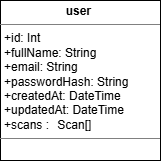
\includegraphics[width=0.3\textwidth]{uploads/diagrams/sprint1classediagram.drawio.png}
    \caption{Class diagram for Sprint 1}
    \label{fig:sprint3-class-diagram}
\end{figure}

\subsection{Sequence Diagram}

The main sequence of this sprint starts when the user submits login credentials from the frontend. The frontend sends the request to the backend, the backend verifies the credentials, and if they are valid, a JWT token is returned and stored locally by the client.

After authentication, every protected request includes the token in the authorization header. The backend middleware checks the token before allowing access to scan creation, scan history, and detailed scan reports. Guest sessions follow the same flow, but the backend blocks access to privileged operations.

The following figure is reserved for the sequence diagram of this sprint.

\begin{figure}[H]
    \centering
    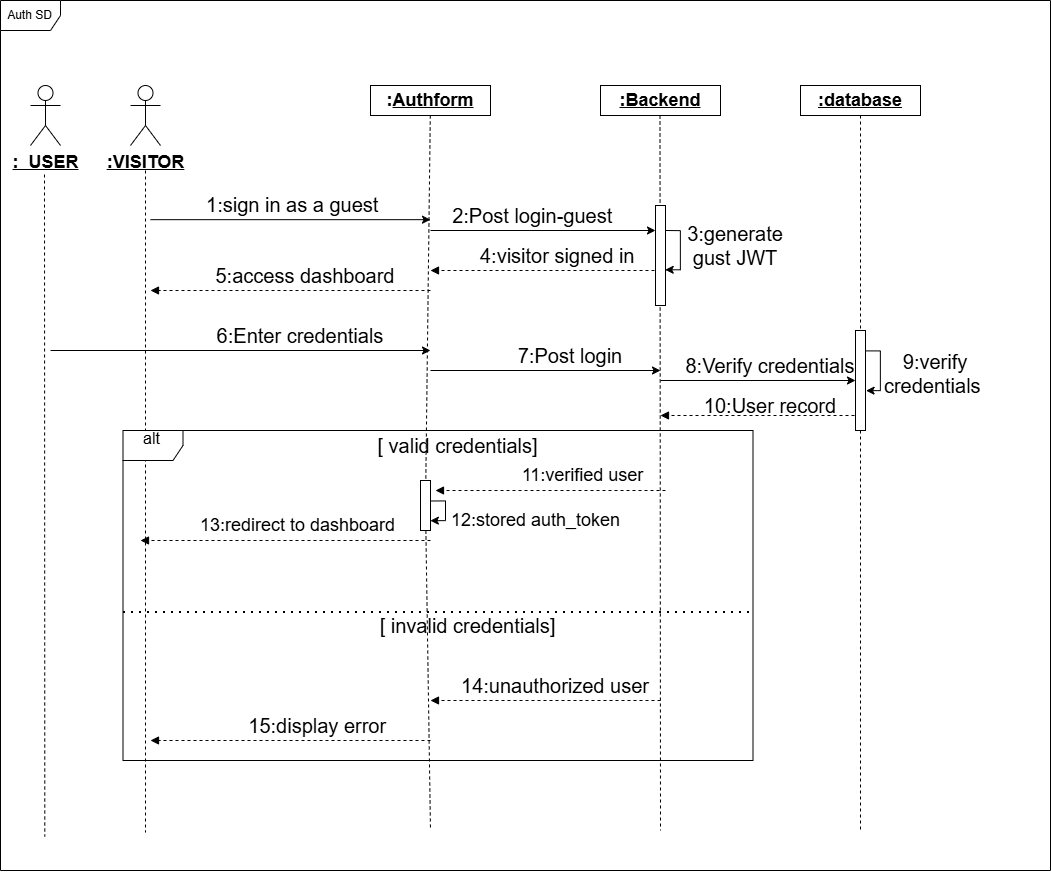
\includegraphics[width=0.98\textwidth]{uploads/diagrams/sprint 1 sequence.drawio.png}
    \caption{Sequence diagram for authentication and access control}
    \label{fig:sprint1-sequence-diagram}
\end{figure}

\section{Implementation}

In this sprint, we present the interfaces developed for Sprint 1. The implementation includes authentication pages (login and registration). The following figures illustrate the application interfaces:

\begin{figure}[H]
    \centering
    \fbox{\parbox{0.85\textwidth}{\centering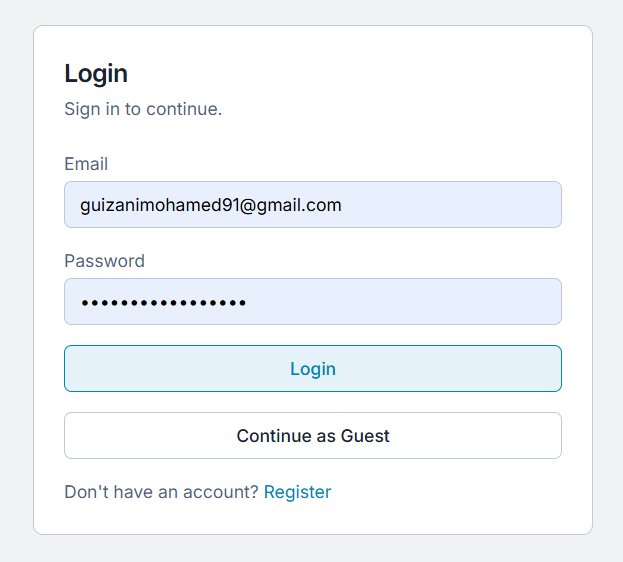
\includegraphics[width=0.85\textwidth]{uploads/images/login.png}}}%
    \caption{Login page}
    \label{fig:login-page}
\end{figure}

\begin{figure}[H]
    \centering
    \fbox{\parbox{0.85\textwidth}{\centering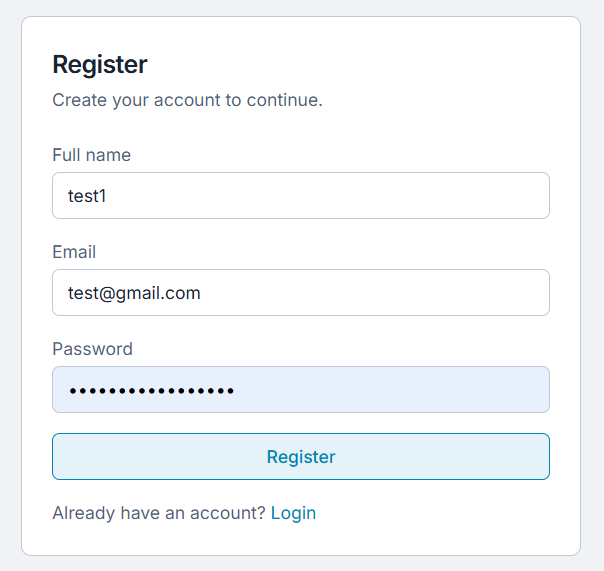
\includegraphics[width=0.85\textwidth]{uploads/images/sign up.png}}}%
    \caption{sign up  page}
    \label{fig:sizgn-up-page}
\end{figure}




 

\section{Conclusion}

This sprint established the authentication and access control layer of the HexStrike platform. It provided a secure login flow, a temporary guest mode, and protected access to sensitive pages and API endpoints.

The next sprint can now focus on the scanning workflow, vulnerability processing, and reporting features on top of this secured foundation.

% -------- Chapter 4 --------
\chapter{Scan Processing Pipeline \& Normalization }
\section{Introduction}

This sprint focuses on the scanning pipeline and on the vulnerability processing features of the HexStrike platform. The goal of this iteration is to implement reliable scan orchestration, normalize heterogeneous tool outputs into a unified schema, match findings against the vulnerability catalog, and persist results for later analysis and reporting.

In practice, this sprint covers scan submission, queueing and scheduling, worker orchestration, normalization, vulnerability matching, result persistence, and the user interfaces to submit and view scans.

\subsection{Sprint Purpose}

The purpose of this sprint is to deliver a robust scan processing pipeline that reliably executes scanners, normalizes their outputs, matches findings to known vulnerabilities, and stores results for retrieval and analysis. Success is measured by correct job processing, normalized result coverage for representative tool outputs, accurate matching to the catalog, and end-to-end retrieval from the UI.

\section{Sprint Backlog}

The backlog for this sprint contains the following user stories:

\begin{table}[H]
    \centering
    \renewcommand{\arraystretch}{1.2}
    \begin{tabularx}{\textwidth}{|X|}
        \hline
        As a user, I can submit a scan target (URL) and receive a job identifier. \\\hline
        As a user, I can schedule or queue scans for later execution. \\\hline
        As the system, I can run scanner tools and collect raw outputs. \\\hline
        As the system, I can normalize raw outputs into a unified \texttt{ScanResult} schema. \\\hline
        As the system, I can match normalized findings to the vulnerability catalog and assign severities. \\\hline
        As a user, I can view, filter, and export scan history and results. \\\hline
        As an operator, I can monitor queue status and worker health. \\\hline
    \end{tabularx}
    \caption{Sprint Backlog}
\end{table}

\section{Requirements Analysis}

\subsection{Use Case Diagram}

The primary actors are the authenticated user (or guest if allowed), the API, and the scan worker. The use case diagram illustrates submission, processing, normalization, matching and viewing flows.

\begin{figure}[H]
    \centering
    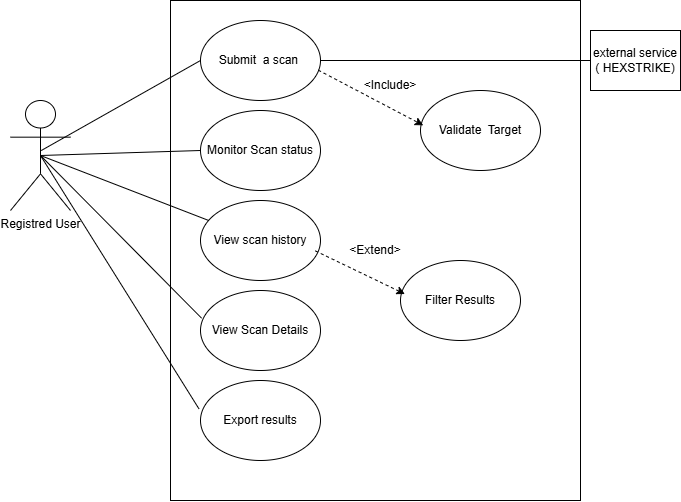
\includegraphics[width=0.9\textwidth]{uploads/diagrams/sprint2 usecas.drawio.png}
    \caption{Use case diagram for scanning and vulnerability processing}
    \label{fig:sprint4-usecase}
\end{figure}

\subsection{Use Case Description}

The main use cases of this sprint are summarized in the following tables.

\begin{table}[H]
    \centering
    \renewcommand{\arraystretch}{1.2}
    \begin{tabular}{|p{3cm}|p{11cm}|}
        \hline
        \textbf{Use case} & Submit Scan \\ \hline
        \textbf{Actor} & Authenticated user (or Guest if permitted) \\ \hline
        \textbf{Description} & The user provides a target (URL) and optional parameters; the backend validates input, creates a \texttt{Scan} job, enqueues it and returns a job identifier. \\ \hline
        \textbf{Pre-condition} & The user is authorized to submit scans and the queue service is available. \\ \hline
        \textbf{Post-condition} & A \texttt{Scan} job is stored and queued for processing; the user receives the job id. \\ \hline
    \end{tabular}
    \caption{Use case description: Submit Scan}
    \label{tab:submit-scan}
\end{table}





\begin{table}[H]
    \centering
    \renewcommand{\arraystretch}{1.2}
    \begin{tabular}{|p{3cm}|p{11cm}|}
        \hline
        \textbf{Use case} & View Scan History \\ \hline
        \textbf{Actor} & Authenticated user \\ \hline
        \textbf{Description} & The user requests a list of past scans, applies filters, and inspects a scan's details and matched vulnerabilities. \\ \hline
        \textbf{Pre-condition} & Scan results have been persisted and the user is authorized to view them. \\ \hline
        \textbf{Post-condition} & The requested data is displayed; the user may export or navigate to details. \\ \hline
    \end{tabular}
    \caption{Use case description: View Scan History}
    \label{tab:view-history}
\end{table}

\begin{table}[H]
    \centering
    \renewcommand{\arraystretch}{1.2}
    \begin{tabular}{|p{3cm}|p{11cm}|}
        \hline
        \textbf{Use case} & View / Browse scan results \\ \hline
        \textbf{Actor} & Authenticated user \\ \hline
        \textbf{Description} & The user selects a completed scan to view its results. The system displays scan metadata including target URL, scan date, scan configuration, and execution summary. It also shows a detailed list of discovered vulnerabilities with severity, affected paths, CVE or reference identifiers, and brief remediation notes. \\ \hline
        \textbf{Pre-condition} & One or more completed scans exist and the user has permission to view them. \\ \hline
        \textbf{Post-condition} & Scan metadata and vulnerabilities are presented to the user; the user may drill down into individual findings or export the data. \\ \hline
    \end{tabular}
    \caption{Use case description: View / Browse scan results}
    \label{tab:view-results-usecase}
\end{table}

\begin{table}[H]
    \centering
    \renewcommand{\arraystretch}{1.2}
    \begin{tabular}{|p{3cm}|p{11cm}|}
        \hline
        \textbf{Use case} & Scan report exporting \\ \hline
        \textbf{Actor} & Authenticated user \\ \hline
        \textbf{Description} & The user requests an export of a completed scan report. The system generates an export file (PDF, CSV or JSON) that includes scan metadata, a summary of findings, detailed vulnerability entries, and optional attachments (screenshots, raw tool outputs). The user can download the file or receive it via email. \\ \hline
        \textbf{Pre-condition} & A completed scan exists and the user has permission to export reports. \\ \hline
        \textbf{Post-condition} & An export file is generated and made available to the user; export operations are logged for audit. \\ \hline
    \end{tabular}
    \caption{Use case description: Scan report exporting}
    \label{tab:scan-export-usecase}
\end{table}

\section{Design}

\subsection{Class Diagram}

The principal components include the API, the queue, worker processes, the normalizer and matcher services, and the persistence layer. The class diagram will show the data models and service classes.

\begin{figure}[H]
    \centering
    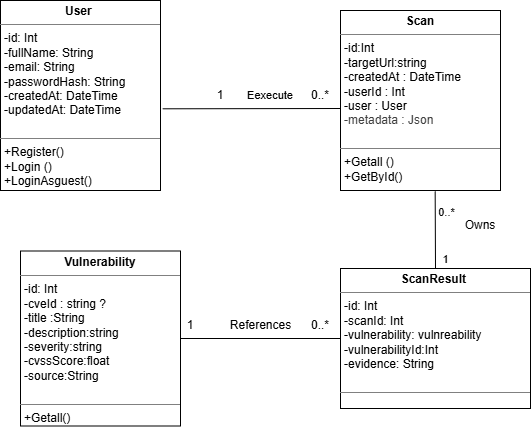
\includegraphics[width=0.98\textwidth]{uploads/diagrams/sprint 2 classe diagram.drawio.png}
    \caption{Class diagram for Sprint 2}
    \label{fig:sprint4-class-diagram}
\end{figure}

\subsection{Scan Workflow}

The scan workflow describes the end-to-end processing of a submitted target: submission, queueing, worker execution of tools, normalization, matching, and persistence. The diagram below summarizes the sequence and components involved.

\begin{figure}[H]
    \centering
    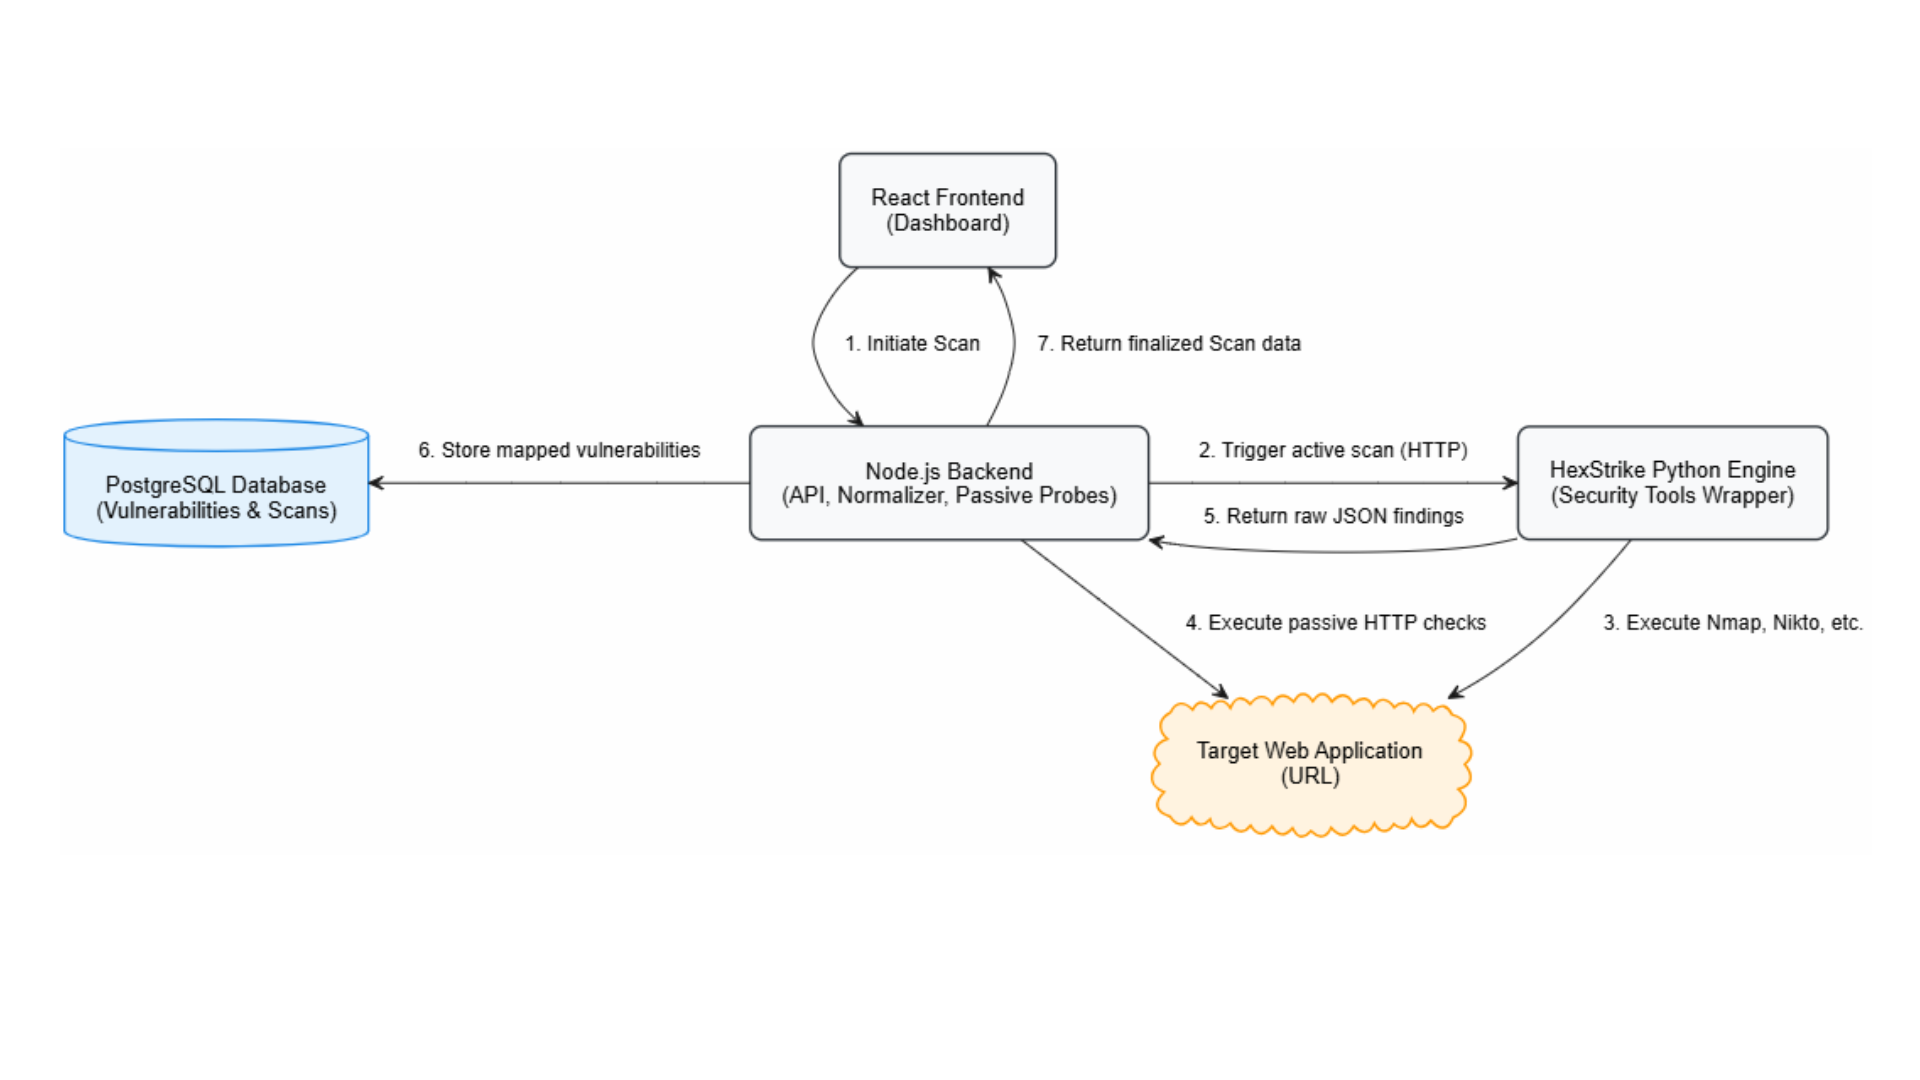
\includegraphics[width=0.9\textwidth]{uploads/diagrams/scan pipline.png}
    \caption{Scan workflow overview}
    \label{fig:scan-workflow}
\end{figure}

\subsection{Sequence Diagram}

Key sequences include submission-to-persistence and normalization-to-matching. A sequence diagram will illustrate the interactions between client, API, queue, worker, normalizer, matcher and DB.

\begin{figure}[H]
    \centering
    
\includegraphics[width=0.98\textwidth]{uploads/diagrams/sprint2 sequence.drawio (3).png}
    \caption{Sequence diagram for scan processing}
    \label{fig:sprint4-sequence-diagram}
\end{figure}

\section{Implementation}

In this sprint, we present the interfaces developed for Sprint 2. The implementation includes the scanner submission interface,  scan history with filtering options, and detailed scan results view. The following figures illustrate the application interfaces:

\begin{figure}[H]
    \centering
    \fbox{\parbox{0.85\textwidth}{\centering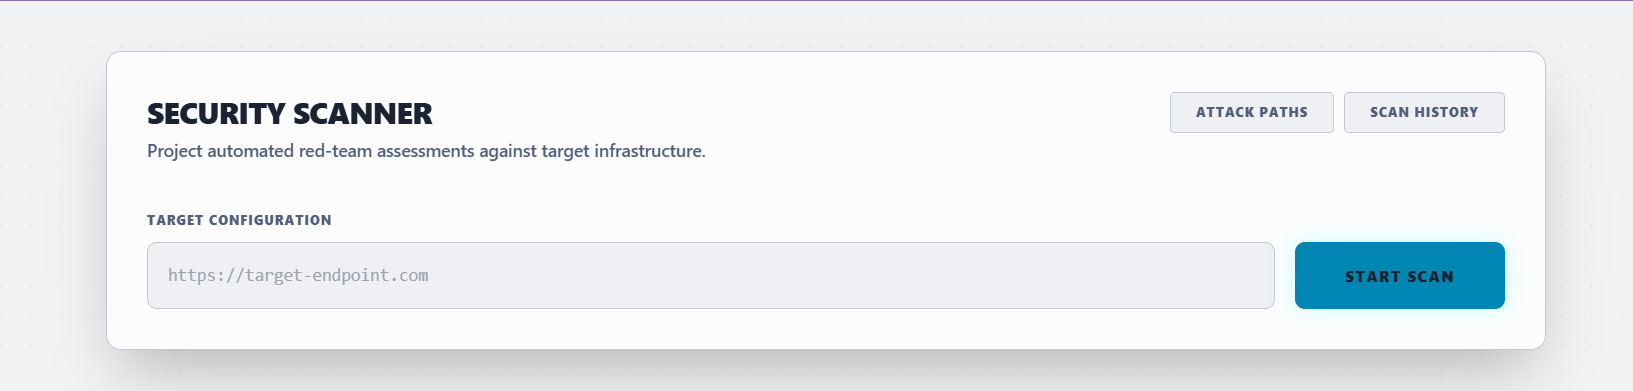
\includegraphics[width=0.85\textwidth]{uploads/images/scan.png}}}% 
    \caption{Scanner submission page}
    \label{fig:scanner4-page}
\end{figure}

\begin{figure}[H]
    \centering
    \fbox{\parbox{0.85\textwidth}{\centering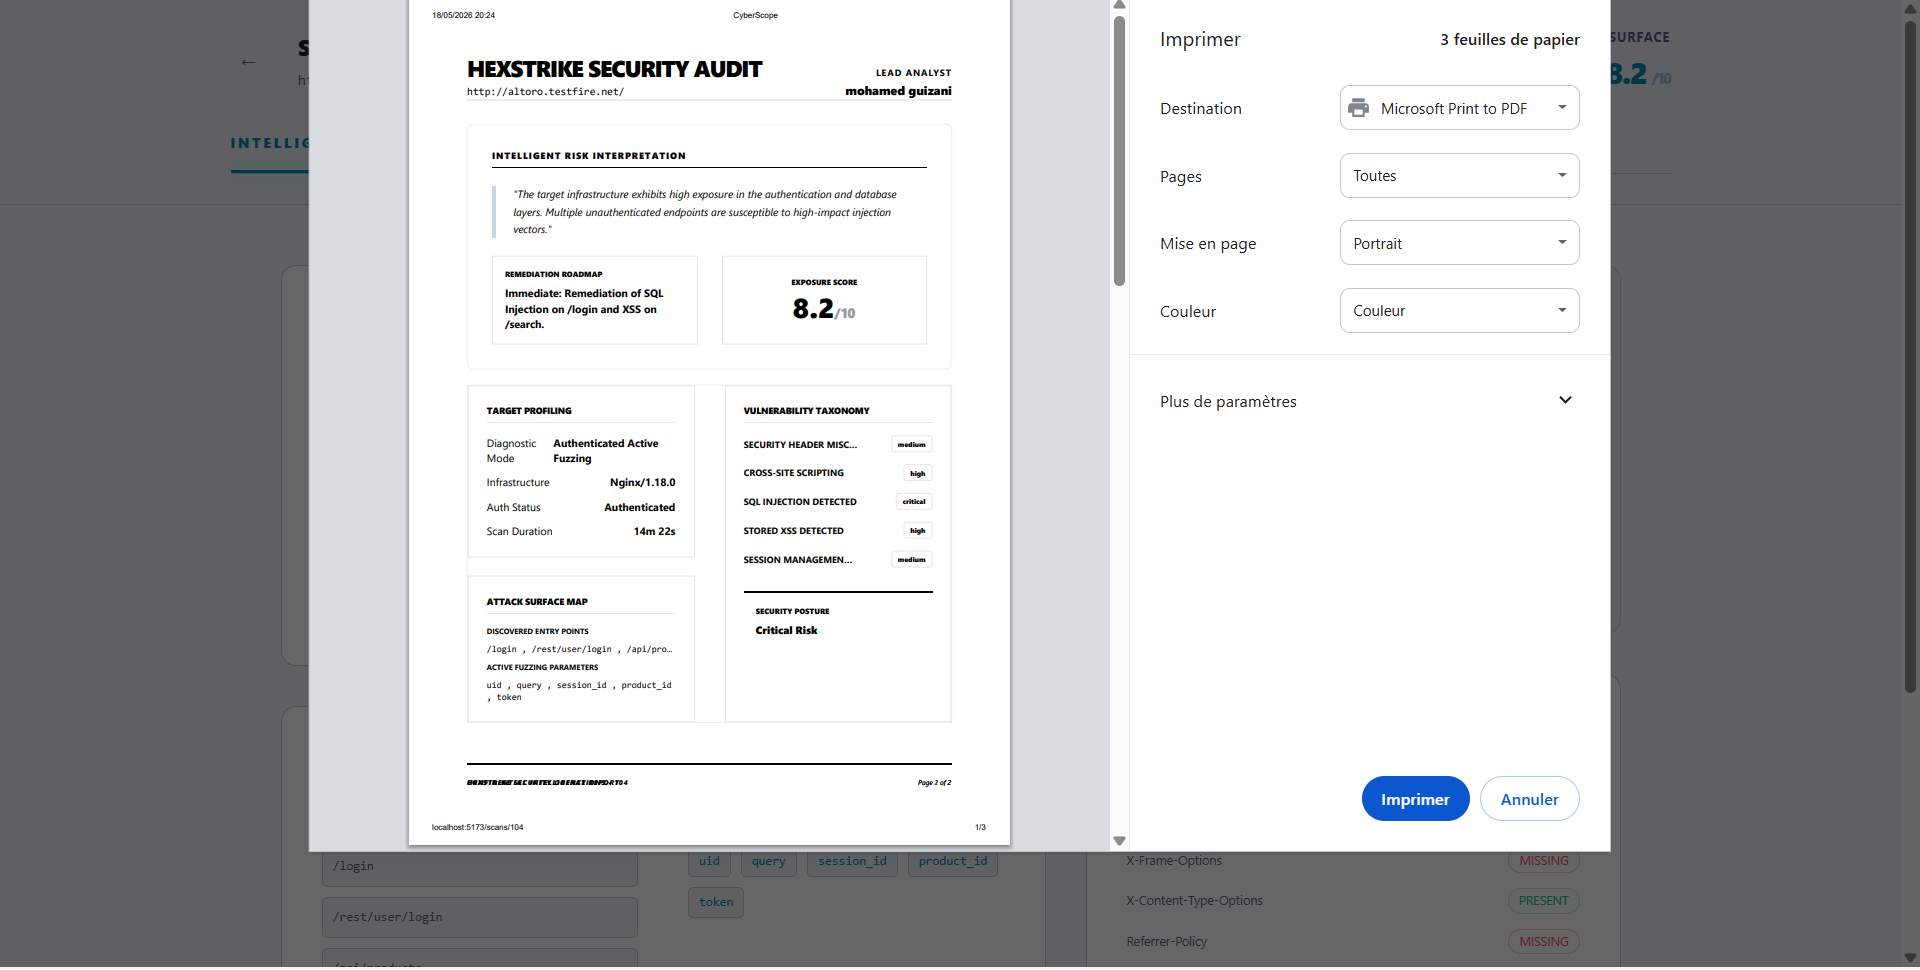
\includegraphics[width=0.85\textwidth]{uploads/images/export.png}}}% 
    \caption{export Scan Report page}
    \label{fig:export-scan-report}
\end{figure}

\begin{figure}[H]
    \centering
    \fbox{\parbox{0.85\textwidth}{\centering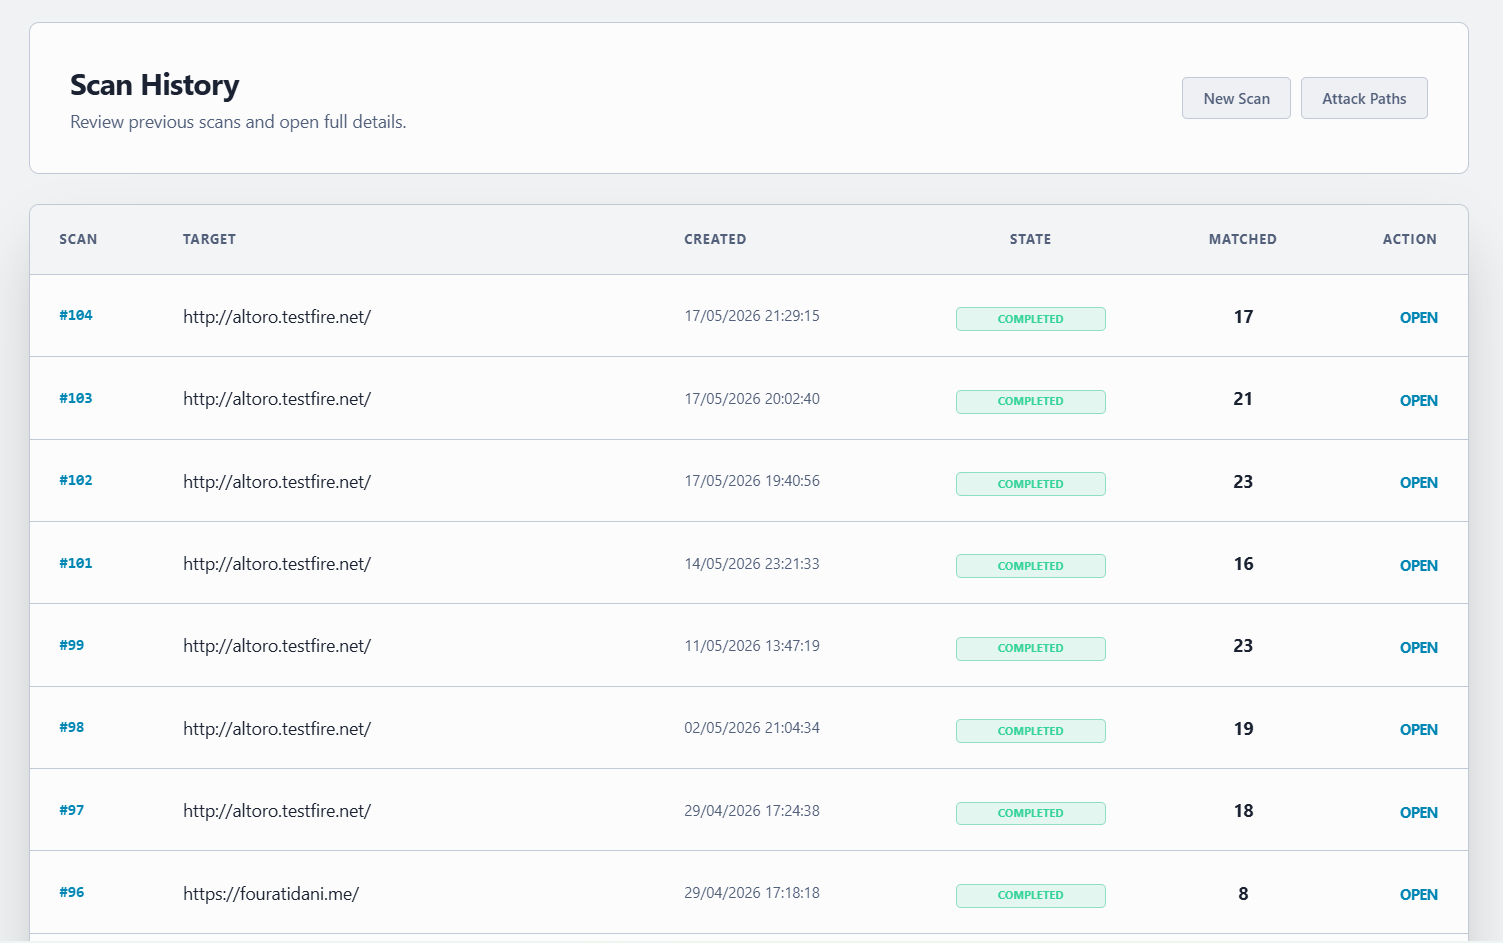
\includegraphics[width=0.85\textwidth]{uploads/images/scan history.png}}}% 
    \caption{Scan history page}
    \label{fig:scan-history4-page}
\end{figure}

\begin{figure}[H]
    \centering
    \fbox{\parbox{0.85\textwidth}{\centering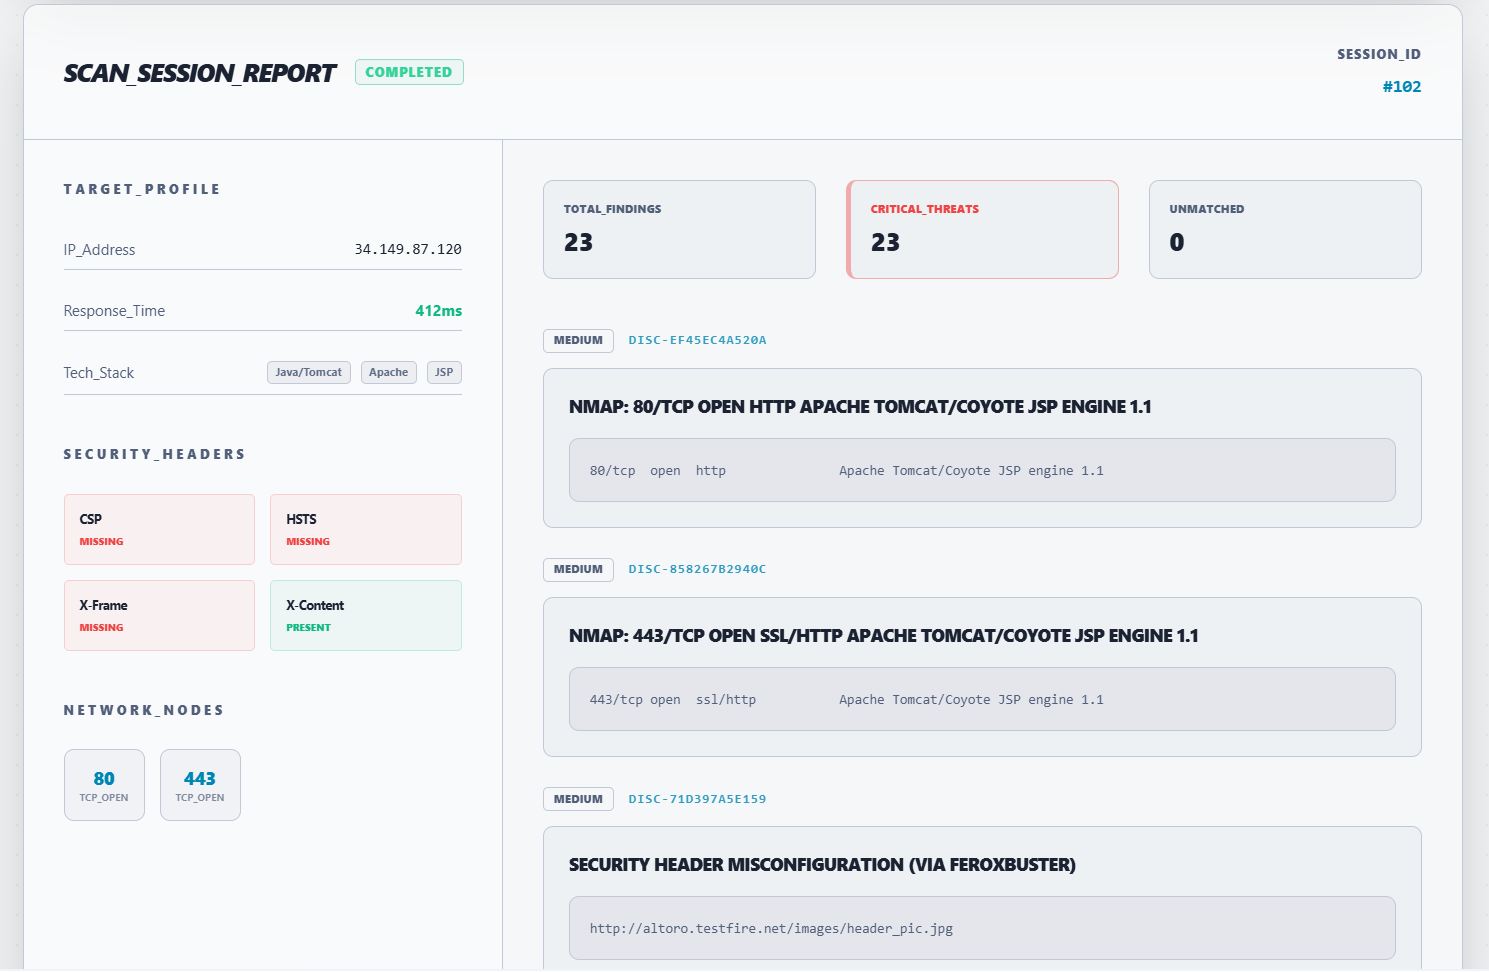
\includegraphics[width=0.85\textwidth]{uploads/images/scan result.png}}}% 
    \caption{Scan details page}
    \label{fig:scan-details4-page}
\end{figure}

\section{Conclusion}

This sprint builds the core scan processing pipeline and the infrastructure to normalize and match findings. With results persisted and accessible through the UI, future sprints can focus on reporting, enrichment, and advanced correlation features.


% -------- Chapter 5 --------
\chapter{Attack Graph Generation }
\section{Introduction}

This sprint is dedicated to attack graph generation. The goal is to transform project artifacts into diagrams that show how data, endpoints and vulnerabilities are connected, so these diagrams highlight potential attack paths in the platform.

\section{Sprint Purpose}

The purpose of this sprint is to implement the Dashboard's attack-path and scenario generation features. The generator is an AI-assisted service that produces ephemeral attack scenarios (ordered steps) and a graph object (nodes and edges) for visualization in the Dashboard. Unlike static report diagrams, these graphs are runtime artifacts produced on-demand and returned to the frontend for interactive rendering.

\section{Sprint Backlog}

The backlog for this sprint focuses on the AI-driven scenario and risk-generation flows and the Dashboard UI integration:

\begin{table}[H]
  \centering
  \renewcommand{\arraystretch}{1.2}
  \begin{tabularx}{\textwidth}{|X|}
    \hline
    As an analyst, I can request an attack scenario for a specific vulnerability and receive structured steps and a graph object. \\\hline
    As an analyst, I can request a risk assessment for a completed scan and receive a summarized JSON assessment. \\\hline
    As the system, I must validate and normalize AI responses into a safe, consistent graph payload (nodes/edges). \\\hline
    As a frontend, the Dashboard should render the returned graph (React Flow) and allow exporting the scenario as JSON. \\\hline
    As an operator, the service should handle AI timeouts, malformed responses, and return useful error messages. \\\hline
  \end{tabularx}
  \caption{Sprint Backlog}
\end{table}

\section{Requirements Analysis}


\subsection{Generation Pipeline}

The generator implements a compact, AI-assisted runtime pipeline: the Dashboard requests a scenario for a selected vulnerability; the backend loads the vulnerability context, builds a controlled prompt, calls the configured AI gateway, extracts and validates the returned JSON, maps normalized steps into an ephemeral graph (nodes and edges), and returns the graph and ordered steps to the frontend for interactive rendering.

\begin{figure}[H]
  \centering
  \fbox{\parbox{0.9\textwidth}{\centering Placeholder: runtime pipeline (Vulnerability/Scan → AI gateway → parser → ephemeral graph)}}
  \caption{Attack graph runtime pipeline (placeholder)}
  \label{fig:graph-pipeline}
\end{figure}

\subsection{Use Case Diagram}

\begin{figure}[H]
  \centering
  \fbox{\parbox{0.85\textwidth}{\centering Placeholder: Use case diagram (select vulnerability → generate scenario → inspect node telemetry)}}
  \caption{Use case diagram for attack-path generation}
  \label{fig:use-case-diagram}
\end{figure}

\section{Design}
\subsection{Graph Data Model}

The attack graph is a simple, on-demand diagram that helps an analyst understand how an attacker could move through the system. It represents a generated scenario as a sequence of human-readable steps — each step has a short title, a clear description of the action, and a note about how serious it is. The diagram shows those steps as boxes connected by arrows to indicate possible flows or next actions. When an analyst clicks a box, the interface shows helpful details and suggested countermeasures for that step.

\subsection{Sequence Diagram (runtime)}

This sequence diagram summarizes the main runtime interaction for on-demand scenario generation: the Dashboard, the backend orchestration service, the AI gateway, and the frontend renderer. It visualizes the request flow (user selection → generation request → AI call → parsing/validation → interactive rendering) and highlights where failures (timeouts, malformed responses) are handled. The diagram emphasizes high-level handoffs rather than implementation details.

\begin{figure}[H]
  \centering
  \fbox{\parbox{0.85\textwidth}{\centering Placeholder: Sequence diagram (Dashboard → Controller → Service → AI → Parser → Dashboard)}}
  \caption{Sequence diagram for runtime scenario generation}
  \label{fig:attack-graph-sequence}
\end{figure}

\section{Implementation}

The implementation focuses on a compact orchestration layer that connects the Dashboard to an AI-based scenario generator while keeping the UI interactive and user-friendly.

- Backend: a lightweight service accepts generation requests, enriches them with vulnerability context, calls the configured AI gateway, and validates and normalizes the returned scenario. The service converts the scenario into an ephemeral graph optimized for client rendering and returns it to the Dashboard. It also handles error conditions (missing records, invalid AI output, gateway timeouts) and surfaces clear HTTP status codes and messages for the frontend to display.

- Frontend: the Dashboard triggers scenario generation for a selected vulnerability, displays progress and error states, and renders the returned graph for interactive inspection. Selecting a node reveals tactical details and suggested countermeasures in the intelligence pane; inventory filters allow analysts to narrow focus before generation.

- Operational notes: generated graphs are ephemeral for this sprint and are not persisted. Raw AI responses are retained only when necessary for debugging and must be protected in production. AI gateway settings (endpoint, model, timeout) are configurable via environment variables and should be tuned for reliability and operator monitoring.

\begin{figure}[H]
  \centering
  \fbox{\parbox{0.85\textwidth}{\centering Placeholder: UI screenshot of Dashboard attack graph rendering}}
  \caption{Dashboard attack graph (placeholder)}
  \label{fig:graph-output}
\end{figure}

\section{Conclusion}

This sprint establishes the attack-graph generation workflow: extraction from source artifacts, enrichment with vulnerability metadata, and rendering to visual formats. The produced graphs will be used in later chapters to illustrate attack paths and support evaluation.


% -------- Chapter 6 --------
\chapter{HexStrike Internals and AI Integration }
\section{HexStrike Internals and AI Integration}

This chapter focuses on HexStrike: its value, internal architecture, and operational details. HexStrike is the orchestration and automation engine that powers tool selection, execution, and intelligent decision making for the project. The chapter highlights how HexStrike complements the CyberScope pipeline, the internals of agent interaction, orchestration, data processing and the AI integration used for risk assessment.

\section{Why HexStrike matters (Value Proposition)}

HexStrike provides a centralized MCP-compatible orchestration layer that coordinates multiple security tools, optimizes parameters using AI, and aggregates results into actionable intelligence. Key benefits are summarized in Table~\ref{tab:feature-benefits} and visualized in Figure~\ref{fig:feature-box}.

\begin{table}[ht]
\centering
\caption{Feature / Benefit summary}
\label{tab:feature-benefits}
\begin{tabularx}{\textwidth}{|l|X|c|}
\hline
Feature & Problem solved & Impact \\
\hline
Automated orchestration & Eliminates manual coordination across tools and brittle scripts & Repeatable runs \\
\hline
AI-assisted selection & Reduces noisy results and manual parameter tuning & Higher precision \\
\hline
Worker scheduling & Mitigates resource contention across workers & Improved throughput \\
\hline
Caching & Avoids re-running identical scans & Lower cost \\
\hline
\end{tabularx}
\end{table}

\begin{figure}[ht]
\centering
\fbox{\parbox[c][4cm][c]{0.85\textwidth}{\centering System component diagram (placeholder) -- replace with real graphic in \texttt{uploads/diagrams/}}}
\caption{High-level component view (placeholder).}
\label{fig:feature-box}
\end{figure}

% Diagrams removed from this chapter; generated visuals will be inserted during final assembly.

\section{Architecture \& Components}

This section lists the main HexStrike components and responsibilities. See Table~\ref{tab:components} for a compact component summary and Figure~\ref{fig:components} for the system diagram.

\begin{table}[ht]
\centering
\caption{Component summary}
\label{tab:components}
\begin{tabularx}{\textwidth}{|l|X|c|}
\hline
Component & Responsibility & Interfaces / Outputs \\
\hline
MCP Server & Task distribution, agent registry & HTTP / gRPC \\
\hline
AI Decision Engine & Tool selection and parameter optimization & Decision API \\
\hline
Worker Manager & Spawn and schedule workers; health monitoring & Worker queue, health API \\
\hline
Cache & Result deduplication and TTL policies & Key-value store \\
\hline
Database & Persist scan results and queries & SQL / REST \\
\hline
UI Connector & Frontend API surface & REST / WebSocket \\
\hline
\end{tabularx}
\end{table}

\begin{figure}[ht]
\centering
\fbox{\parbox[c][4cm][c]{0.85\textwidth}{\centering Component diagram (placeholder) -- replace with exported diagram}}
\caption{HexStrike component diagram (placeholder).}
\label{fig:components}
\end{figure}

\section{Agent Interaction \& MCP Protocol}

Agents connect to HexStrike using the MCP protocol. They register capabilities, receive tasks, and stream results back. A swimlane-style sequence (Agent / MCP / Worker / Tool) captures registration, task assignment, execution and streaming of results; include an illustrated diagram only if needed.

% Sequence diagram removed: kept concise textual description above.

\section{Tool Orchestration \& Execution Flow}

Tool orchestration covers discovery, selection by the decision engine, execution scheduling, retries and fallback strategies. The text summarizes decision points and parallel execution branches; include a flowchart only when a visual is required for reviewers.

% Orchestration flowchart removed to reduce figures; see Table~\ref{tab:components} and the textual description.

\section{Data Pipeline: Normalization, Matching \& Enrichment}

Raw scanner outputs are transformed into structured \texttt{ScanResult} objects, matched against a vulnerability catalog, and enriched with CVE and CVSS data. Table~\ref{tab:schema} gives a short schema fragment and Figure~\ref{fig:dataflow} shows the data flow.

\begin{table}[ht]
\centering
\caption{Key fields in \texttt{ScanResult} (example)}
\label{tab:schema}
\begin{tabularx}{\textwidth}{|l|l|X|}
\hline
Field & Type & Description \\
\hline
id & string & Unique identifier for the finding \\
\hline
source & string & Tool that produced the finding \\
\hline
evidence & object & Raw evidence and context (headers, request/response) \\
\hline
severity & string & Normalized severity (low/medium/high) \\
\hline
references & array & CVE ids and external links \\
\hline
\end{tabularx}
\end{table}

\begin{figure}[ht]
\centering
\fbox{\parbox[c][3.5cm][c]{0.85\textwidth}{\centering Data pipeline / ER diagram (placeholder)}}
\caption{Data pipeline and entity relationships (placeholder).}
\label{fig:dataflow}
\end{figure}

\section{Process Management, Caching \& Error Recovery}

HexStrike employs process-level state management for workers and a caching layer to avoid re-running expensive scans. Error recovery strategies include exponential backoff, automatic retries, and fallback scanning behaviors. Table~\ref{tab:retry} summarizes retry/backoff policies; include a worker state diagram only if visual clarification is needed.

\begin{table}[ht]
\centering
\caption{Retry/backoff policy (example)}
\label{tab:retry}
\begin{tabular}{|l|l|l|}
\hline
Condition & Action & Notes \\
\hline
Transient network error & Retry up to 3 times & Exponential backoff: 2s, 4s, 8s \\
\hline
Tool timeout & Retry once with increased timeout & Log and escalate after failure \\
\hline
Permanent error & Mark failed & Store diagnostics for analyst \\
\hline
\end{tabular}
\end{table}

% Worker state machine figure removed; see Table~\ref{tab:retry} for policy summary.

\section{Conclusion}

HexStrike acts as the project's orchestration backbone. The architecture and internal workflows presented in this chapter demonstrate how the system automates complex multi-tool assessments and provides higher-level intelligence to reduce analyst workload.

% -------------------- REFERENCES --------------------
\clearpage
\renewcommand{\bibname}{References}
% Tweak spacing for the References page to increase vertical gaps
\begingroup
\setlength{\parskip}{6pt}
\renewcommand{\baselinestretch}{1.10}\selectfont
\bibliographystyle{ieeetr}
% Force inclusion of project-related references that are not \cite'd in text
\nocite{nmap,ollama,reactflow,jwt,chromium,hexstrike,sqlmap,nuclei,nikto,owasp,zap,burp,stackhawk,detectify,snyk,ibm_breach_2024,verizon_dbir_2024,prisma,vite,react,typescript}
\bibliography{references}
\endgroup

% -------------------- CONCLUSION --------------------
\clearpage
\chapter*{General Conclusion}
\addcontentsline{toc}{chapter}{General Conclusion}
\markboth{General Conclusion}{General Conclusion}
This report has presented the analysis, design, and implementation of CyberScope, an integrated platform for automated web application security assessment. We described the adopted development methodology, the system architecture, the orchestration of external scanning tools, and the frontend dashboard used for visualization and reporting. The work demonstrates how heterogeneous components—backend services, a Python-based scanning engine, dynamic crawlers, and AI-assisted analysis—can be combined into a coherent, extensible solution.

The implementation validated the proposed architecture: the backend provides reliable orchestration and persistence of scan results, the scanning engine automates interactions with established security tools, and the frontend offers clear visualization and filtering of findings. Key design choices such as modularity, use of standard tooling (Node.js, Prisma, PostgreSQL, React), and the adoption of an orchestration layer (HexStrike AI) made the system easier to extend and maintain.

Evaluation focused on correctness, scalability and usability. The pipeline successfully aggregates heterogeneous outputs, normalizes and deduplicates findings, and produces structured reports that facilitate prioritization and remediation. Performance considerations and fault-tolerance mechanisms were discussed to ensure scans can run concurrently and recover from partial failures. Usability improvements in the dashboard and report generation help stakeholders rapidly understand the security posture of target applications.

Future work includes broadening tool coverage, improving the AI analysis models and integration (e.g., richer local models or external engines), adding role-based access control and audit trails, and hardening the orchestration layer for large-scale distributed scans. Additional validation in realistic production scenarios and user studies would further strengthen the platform's maturity and operational readiness.

In summary, CyberScope provides a pragmatic and extensible foundation for automated web application security assessment. The project combines proven open-source tools, a maintainable development stack, and automation patterns that together enable efficient, repeatable security testing and reporting for modern web applications.

\end{document}